% Main file. MDPI ACS template, Electronics submission mode.
% Author details and funding statement supplied by the authors.
\documentclass[electronics,article,submit,moreauthors]{Definitions/mdpi}
\errorcontextlines=80
% Do not modify the supplied mdpi.cls. Use its unchanged vector logo in PDF
% format so that sandboxed Tectonic/XeTeX does not need EPS shell conversion.
\let\MDPIOriginalIncludeGraphics\includegraphics
\renewcommand{\includegraphics}[2][]{%
  \IfStrEq{#2}{Definitions/logo-mdpi.eps}%
    {\MDPIOriginalIncludeGraphics[#1]{Definitions/logo-mdpi.pdf}}%
    {\MDPIOriginalIncludeGraphics[#1]{#2}}%
}

% Add the official journal logo while retaining the template's submit mode.
\makeatletter
\patchcmd{\@maketitle}{\hfill \href{https://www.mdpi.com}}{\href{https://www.mdpi.com/journal/electronics}{
\includegraphics[height=1cm]{Definitions/electronics-logo.png}}\hfill \href{https://www.mdpi.com}}{}{\PackageError{electronics-header}{Journal logo insertion failed}{Check the MDPI title-header definition.}}
\makeatother
\usepackage[ruled,vlined,linesnumbered,algo2e]{algorithm2e}
\SetAlFnt{\small}
\SetAlCapFnt{\small\bfseries}
\SetAlCapNameFnt{\small\bfseries}
\SetAlgoNlRelativeSize{-1}
\SetNlSty{textnormal}{}{}
\DontPrintSemicolon
\newcommand{\FullSuccess}{30}
\newcommand{\FullCPUMean}{2.65}
\newcommand{\FullCPUSD}{0.17}
\newcommand{\FullCPUMedian}{2.51}
\newcommand{\FullCPUPninetyfive}{5.67}
\newcommand{\FullCPUMaximum}{8.78}
\newcommand{\FullWallMean}{2.43}
\newcommand{\FullWallSD}{0.12}
\newcommand{\FullWallMedian}{2.57}
\newcommand{\FullWallPninetyfive}{3.43}
\newcommand{\FullWallMaximum}{6.21}
\newcommand{\StraightSuccess}{7}
\newcommand{\StraightCPUMean}{14.40}
\newcommand{\StraightCPUSD}{0.88}
\newcommand{\StraightCPUMedian}{13.05}
\newcommand{\StraightCPUPninetyfive}{29.24}
\newcommand{\StraightCPUMaximum}{31.36}
\newcommand{\StraightWallMean}{15.17}
\newcommand{\StraightWallSD}{0.56}
\newcommand{\StraightWallMedian}{13.74}
\newcommand{\StraightWallPninetyfive}{30.70}
\newcommand{\StraightWallMaximum}{31.19}
\newcommand{\HardSuccess}{29}
\newcommand{\HardCPUMean}{1.86}
\newcommand{\HardCPUSD}{0.10}
\newcommand{\HardCPUMedian}{1.83}
\newcommand{\HardCPUPninetyfive}{3.63}
\newcommand{\HardCPUMaximum}{5.94}
\newcommand{\HardWallMean}{1.65}
\newcommand{\HardWallSD}{0.10}
\newcommand{\HardWallMedian}{1.79}
\newcommand{\HardWallPninetyfive}{2.59}
\newcommand{\HardWallMaximum}{2.80}

\firstpage{1}
\pubvolume{1}\issuenum{1}\articlenumber{0}
\pubyear{2026}\copyrightyear{2026}
\datereceived{ }\daterevised{ }\dateaccepted{ }\datepublished{ }
\Title{Feasibility Recovery for Fixed-Horizon Multi-UAV Cooperative Flight Trajectory Optimization in High-Conflict Regions}
\Author{Yangfan Liu $^{1}$, Ziqing Ye $^{2}$, Biao Qian $^{3}$, Wei Tian $^{4,*}$ and Zhonghong Wu $^{3}$}
\AuthorNames{Yangfan Liu, Ziqing Ye, Biao Qian, Wei Tian and Zhonghong Wu}
\address{%
$^{1}$ \quad College of Shipbuilding Engineering, Harbin Engineering University, Qingdao 266000, China; 2020010115@hrbeu.edu.cn\\
$^{2}$ \quad Unit 92728 of the People's Liberation Army of China, Shanghai 201901, China; 354700311@qq.com\\
$^{3}$ \quad College of Weaponry Engineering, Naval University of Engineering, Wuhan 430033, China; 2799825233@qq.com (B.Q.); 1714001017@nue.edu.cn (Z.W.)\\
$^{4}$ \quad School of Information and Electronic Engineering, East China Normal University, Shanghai 200241, China}
\corres{Correspondence: wtian@cee.ecnu.edu.cn}
\newcommand{\R}{\mathbb{R}}
\newcommand{\norm}[1]{\left\lVert #1\right\rVert}
\newcommand{\bx}{\mathbf{x}}
\newcommand{\bp}{\mathbf{p}}
\newcommand{\bv}{\mathbf{v}}
\newcommand{\ba}{\mathbf{a}}
\newcommand{\one}{\mathbf{1}}
\DeclareMathOperator{\geomdist}{dist}
\DeclareMathOperator{\vecop}{vec}
\DeclareMathOperator{\clip}{clip}
\newcolumntype{Y}{>{\raggedright\arraybackslash}X}
\setlength{\emergencystretch}{2em}
\brokenpenalty=10000
\setlength{\headheight}{19pt}
% Full-width scientific figures may share a page with a short text block.
\renewcommand{\topfraction}{0.9}
\renewcommand{\bottomfraction}{0.9}
\renewcommand{\textfraction}{0.08}
\renewcommand{\floatpagefraction}{0.75}
% Working draft: no assigned DOI and no claim that submission has occurred.
\renewcommand{\cright}{\mbox{}}
\fancypagestyle{plain}{\fancyhf{}\renewcommand{\headrulewidth}{0pt}\renewcommand{\footrulewidth}{0.4pt}\fancyfoot[L]{\footnotesize Manuscript for \emph{Electronics}}\fancyfoot[R]{\footnotesize\thepage}}
\AtBeginDocument{\fancyhead[L]{\footnotesize Manuscript for \emph{Electronics}}\fancyhead[R]{\footnotesize\thepage{} of \pageref*{LastPage}}\fancyfoot[L]{}\fancyfoot[R]{}}
\abstract{Cooperative flight through high-conflict regions requires multiple unmanned aerial vehicles to reconcile obstacle clearance, mutual separation, and motion limits within a prescribed completion time. This paper develops a lightweight iterative optimization method for feasibility recovery in fixed-horizon cooperative trajectory planning. A double-integrator model and spatial and relative corridors yield convex quadratic subproblems. Separate penalties on affine kinematic defects and relative-box violations preserve subproblem nonemptiness under endpoint-compatible spatial boxes, while static free-space and translational motion bounds remain hard constraints. A synchronized geometric reference initializes the process. Capped penalty updates and corridor reconstruction maintain intermediate candidates and support consistency recovery without extending the flight horizon. After numerical recovery, closed-form endpoint control correction and exact integration produce continuous-velocity rest-to-rest motion. Complete-interval clearance and motion-limit checks determine final acceptance. Controlled simulations evaluate guided initialization, task-matched computational baselines, and recovery under reduced flight time and corridor freedom. The results demonstrate second-scale planning for the tested small teams and an expanded acceptance region under restricted local geometry, linking tractable optimization to recovery of fixed-horizon cooperative motion.}
\keyword{relative safe corridor; lightweight iterative optimization method (LIOM); trajectory planning; cooperative trajectory planning; computational optimal control}
\begin{document}
\section{Introduction}
Cooperative trajectory planning enables multiple unmanned aerial vehicles (UAVs) to execute coordinated missions in a shared three-dimensional workspace. When several vehicles approach an intersection or a narrow passage, their trajectories must satisfy obstacle clearance, mutual separation, and motion limits simultaneously. Aerial-swarm research has established the importance of these coupled requirements~\cite{chung2018}, while agile quadrotor teams and coordinated formation transitions demonstrate their practical relevance~\cite{kushleyev2012,preiss2017}. Recent work combines three-dimensional reciprocal velocity obstacles with multi-agent reinforcement learning to coordinate collision avoidance within structured urban airspace~\cite{zhong2025rvo}.

Computational efficiency is essential when a feasible coordinated motion must be obtained within a limited planning interval. Enhanced sequential convex programming has been integrated with model predictive control to address formation tracking and correct linearization errors that can compromise feasibility~\cite{liu2025escp}. Conflict-free multi-robot planning coupled with predictive control connects coordination decisions to feasible motion~\cite{wu2025conflict}. Cooperative exploration combines dynamic Voronoi partitioning with learned obstacle avoidance~\cite{zhao2025exploration}, while multi-UAV coverage planning jointly considers task allocation and travel time under repeated round-trip operation~\cite{li2025coverage}. Together, these studies motivate methods that account for coupled coordination, safety, and timing requirements while keeping computation manageable.

High-conflict regions arise where assigned routes intersect or several UAVs compete for a shared passage around obstacles. Safe corridors express collision avoidance through conservative linear restrictions. A useful reference can nevertheless produce local corridors that conflict with one another or with bounded motion. Under a prescribed completion time, all of these requirements must be reconciled within the original flight horizon. A failed local solve therefore calls for a mechanism that can revise the coordinated motion and its surrounding geometry while preserving the task boundaries.

This paper develops a lightweight iterative optimization method (LIOM) for fixed-horizon, rest-to-rest cooperative flight. The double-integrator model and fixed spatial and relative corridors give a convex quadratic structure. Separate penalties on kinematic defects and relative-box violations allow intermediate candidates to reshape the corridors while retaining hard static free-space and translational motion bounds. A synchronized reference initializes the process. Bounded penalty updates support numerical recovery, and a closed-form endpoint control correction connects recovered candidates to continuous-velocity motion over the prescribed horizon.

The main contributions are twofold:
\begin{enumerate}
\item A fixed-horizon recovery formulation reconciles prescribed rest-to-rest states with spatial and relative collision-avoidance regions. The affine model and corridor constraints retain a convex quadratic subproblem, whose nonemptiness is established by an explicit feasible-point construction under endpoint-compatible spatial boxes. This formulation permits continued local refinement through temporary incompatibilities among kinematics, static avoidance, and mutual separation.
\item A closed-form endpoint control correction connects numerical recovery to continuous-velocity motion with the prescribed boundary states. Exact integration is followed by complete-interval clearance and motion-limit checks on the reconstructed trajectory; these checks determine final acceptance. The procedure retains the original flight horizon and requires no additional iterative optimization solve for endpoint correction.
\end{enumerate}
Simulation studies evaluate accepted cooperative motions, computation time, and the role of initialization. Task-matched comparisons and controlled pressure sweeps examine how local geometric restrictions and recovery affect success within a fixed flight horizon.

\section{Related Work}
\label{sec:related}
\subsection{Coordinated Paths and Predictive Trajectory Planning}
Cooperative planning requires both a compatible passing pattern and motions that vehicles can execute. Preiss et al.~\cite{preiss2017} combined discrete coordination with polynomial refinement and downwash-aware separation. H\"onig et al.~\cite{hoenig2018} used collision-annotated roadmaps to connect multi-agent path finding to continuous quadrotor trajectories. CAPT~\cite{turpin2014} jointly selects assignments and trajectories for interchangeable robots. These approaches exploit discrete coordination to resolve conflicts before continuous refinement. For prescribed assignments and arrival times, the refinement stage must additionally reconcile the selected routes with the available motion budget.

Distributed model predictive control (MPC) resolves interactions through predicted neighbor motions. Luis and Schoellig~\cite{luis2019} introduced on-demand collision constraints and penalized relaxation; Luis et al.~\cite{luis2020} developed online trajectory generation with continuous input parameterization and event-triggered replanning. Buffered Voronoi cells~\cite{zhou2017bvc} instead allocate local free space through relative-position geometry. Communication-efficient predictive formation control~\cite{schiz2025communication} reduces exchanged information using autoencoders. Prediction, local geometric separation, and communication reduction address different computational bottlenecks. Predictive schemes use rolling decision horizons to support online operation, whereas a prescribed common completion time couples the entire remaining motion to its terminal boundary conditions.

\subsection{Safety Filters and Deadlock-Aware Control}
Control barrier functions (CBFs) offer an alternative to repeated full-trajectory planning. Gon\c{c}alves et al.~\cite{goncalves2024} generated drone acceleration fields through a CBF-based quadratic program (QP), followed by thrust and angular-velocity tracking. Their construction provides safety, motion-limit, and QP-feasibility results under its stated conditions. Mestres et al.~\cite{mestre2024} distributed a coupled CBF optimization using auxiliary constraint-mismatch variables, with safety and asymptotic optimality properties for the state-dependent control problem. The optimized quantity in these filters concerns the current control action; a complete trajectory satisfying a prescribed rest-to-rest deadline requires an additional temporal coordination mechanism.

Safe local actions can also encounter coordination deadlocks. Grover et al.~\cite{grover2023} characterized deadlock through the optimality conditions of reactive controllers and developed resolution strategies for two- and three-robot configurations. Jankovic et al.~\cite{jankovic2024} connected gridlock propensity to equilibrium stability and established feasibility for centralized and selected co-optimization policies. Their predictor--corrector strategy illustrates how sharing the responsibility for avoidance improves progress. Chandra et al.~\cite{chandra2025} integrated discrete-time CBFs and deadlock prevention into decentralized receding-horizon optimal control. These developments explicitly address safety and progress, but their navigation formulations do not impose the fixed common rest-to-rest completion task considered here. The relevant distinction is the temporal scope of recovery: local admissible control and eventual progress must be complemented by compatibility with the remaining flight time.

\subsection{Corridors, Motion Limits, and Trajectory Commitment}
Corridors reduce geometric collision restrictions to tractable local constraints. Spatial and relative constructions organize static and mutual avoidance within cooperative optimization~\cite{bu2025}. Park and Kim~\cite{park2021} used relative safe flight corridors to account for uncertain obstacle motion, with slack and reciprocal avoidance to relax their local restrictions. These mechanisms address an important weakness of hard separating corridors: collision-free local regions can still have no intersection with the motions permitted by dynamics and endpoint conditions. A QP solver cannot resolve that geometric incompatibility by optimizing more accurately. Their online formulation updates predictions and avoidance responsibilities; a fixed common arrival time additionally requires recovery of the full rest-to-rest motion within the remaining time allocation. \c{S}enba\c{s}lar et al.~\cite{senbaslar2023} developed RLSS, a networkless planner using linear spatial separations and piecewise-polynomial QPs. RLSS checks derivative limits after optimization and increases segment durations when necessary. Prescribing the completion horizon removes this temporal adjustment and places the recovery burden on motion and geometry.

Online planners also emphasize trajectory commitment and communication. EGO-Swarm~\cite{zhou2021ego} combines local trajectory optimization with perception and implicit topological alternatives. MADER~\cite{tordesillas2022} optimizes trajectories and separating planes with asynchronous check--recheck commitment; Robust MADER~\cite{kondo2024} extends this strategy to communication delays. PRIMER~\cite{kondo2025} learns perception-aware position--yaw planning while retaining deconfliction. Park et al.~\cite{park2025} combine multi-agent waypoints and subgoal optimization, with goal-convergence guarantees in static environments under fully connected communication and deadlock prevention under limited communication. These results establish substantial online coordination capabilities. The present setting focuses on another requirement: returning jointly accepted motions for all assigned UAVs at an unchanged common deadline, including when initial corridor choices conflict with motion constraints.

\subsection{Centralized Cooperative Optimization and Recovery}
Centralized optimization directly couples the motions of interacting vehicles. Adaptive-scaling constrained optimization (ASCO)~\cite{li2021asco} reduces a nonholonomic cooperative planning problem by selecting collision constraints within an adjustable risk range. Failed intermediate solves trigger range contraction, while detected violations expand the active range. The approach therefore includes a recovery mechanism, although its intermediate problems retain nonlinear vehicle dynamics and optimize the terminal time. For the double-integrator task studied here, affine defects and fixed corridor geometry permit convex QPs; box-separation bounds also identify pair restrictions that are unnecessary throughout the current spatial boxes.

Priority-sharing autonomous intersection management~\cite{li2023priority} combines parameterized social-force references, nonlinear cooperative optimization, and batch reservations. Its fixed-duration traverse stage terminates on exit regions, and unsuccessful optimization can lead to a smaller cooperative batch, ultimately a single vehicle. The present recovery task retains the specified team, fixed terminal positions, and rest-to-rest states throughout joint refinement. This boundary-condition commitment concentrates the remaining flexibility in the coordinated motions. It also explains the role of the reference: it supplies a useful passing pattern, while optimization must resolve its remaining incompatibilities.

Sequential convex programming replaces nonlinear separation constraints by local affine restrictions and updates the expansion trajectories~\cite{augugliaro2012}. This yields tractable subproblems, but a chosen linearization can exclude every trajectory compatible with hard motion and endpoint constraints. Enhanced sequential convex programming~\cite{liu2025escp} addresses accumulated linearization errors in predictive formation tracking. In the present model, the integration defects are affine. Softening preserves access to intermediate candidates when current geometric restrictions conflict with exact integration. The fixed-horizon formulation retains this convex structure while endpoint control moments connect recovered candidates to physically checked motion.

\subsection{Fixed-Horizon Feasibility Recovery}
Table~\ref{tab:distinction} compares the decision scope, timing assumptions, and feasibility mechanisms of representative methods. The present task keeps the team, terminal states, and common arrival time fixed. Its central difficulty is compatibility: individually admissible spatial and relative regions can jointly exclude every motion satisfying exact integration. The proposed formulation preserves intermediate candidates through separate kinematic and relative-box penalties, uses them to reconstruct local corridors, and recovers endpoint-consistent controls before complete-interval acceptance. This connects local optimization to the full fixed-horizon task while retaining hard free-space and componentwise motion restrictions.

\begin{table}[htbp]
\begin{adjustwidth}{-\extralength}{0cm}
\caption{Methodological distinctions among representative cooperative planning and safety-control formulations. A prediction horizon specifies a local planning window; a completion horizon specifies the task's arrival time.\label{tab:distinction}}
\small\setlength{\tabcolsep}{4pt}\renewcommand{\arraystretch}{1.15}
\begin{tabularx}{\fulllength}{>{\raggedright\arraybackslash}p{2.65cm}>{\raggedright\arraybackslash}p{3.35cm}>{\raggedright\arraybackslash}p{3.15cm}Y}
\toprule
Method & Coordination and geometry & Time and motion limits & Feasibility or safety mechanism \\
\midrule
ASCO~\cite{li2021asco} & Centralized nonlinear trajectories; selected distance constraints & Optimized terminal time; hard motion bounds & Adapts the active risk range after failed solves or constraint violations; checks the full discretized constraints. \\
\addlinespace[3pt]
Park and Kim~\cite{park2021} & Online polynomial QP; relative safe flight corridors & Receding horizon; derivative bounds in QP & Relative-corridor relaxation and reciprocal avoidance address prediction uncertainty; convex-hull restrictions cover trajectory segments. \\
\addlinespace[3pt]
RLSS~\cite{senbaslar2023} & Decentralized polynomial QP; spatial separating planes & Adjustable durations; derivative limits checked afterward & Geometric separation protects the executed portion; temporal rescaling restores derivative limits when needed. \\
\addlinespace[3pt]
Priority-sharing AIM~\cite{li2023priority} & Centralized nonlinear optimization; social-force initialization & Fixed traverse duration; hard motion bounds & Reservation and batch reduction handle unresolved conflicts; terminal positions lie on exit regions. \\
\addlinespace[3pt]
Gon\c{c}alves et al.~\cite{goncalves2024} & Centralized CBF-QP acceleration field & Instantaneous control; speed and acceleration limits & Feasible safety-filter construction and acceleration tracking under the stated assumptions; no prescribed common arrival time. \\
\addlinespace[3pt]
Mestres et al.~\cite{mestre2024} & Distributed state-dependent CBF optimization & Instantaneous control; waypoint navigation & Constraint-mismatch coordination preserves safety with asymptotic control-optimality properties; no full-horizon endpoint recovery. \\
\addlinespace[3pt]
Jankovic et al.~\cite{jankovic2024} & CBF-QP control; centralized and decentralized policies & Instantaneous acceleration selection & Feasibility analysis and predictor--corrector coordination address collision avoidance and liveness; no common task deadline. \\
\addlinespace[3pt]
Robust MADER~\cite{kondo2024} & Decentralized polynomial planning; separating planes & Receding planning; dynamic limits & Delay-aware trajectory commitment preserves safety despite communication delay. \\
\addlinespace[3pt]
Chandra et al.~\cite{chandra2025} & Decentralized MPC with discrete-time CBFs & Receding horizon; state and input constraints & Liveness-set constraints prevent deadlock in social navigation; safety is imposed through discrete-time barriers. \\
\addlinespace[3pt]
SCP~\cite{augugliaro2012} & Centralized trajectory optimization; local affine separation restrictions & Prescribed trajectory duration; motion constraints & Successive local convex approximations and vehicle-specific feasibility checking. \\
\addlinespace[3pt]
\textbf{Proposed LIOM} & Centralized QP; spatial and relative boxes & Fixed common horizon and endpoints; hard component bounds & Separate penalties preserve intermediate candidates; corridor rebuilding, endpoint control correction, and complete-interval checking recover and accept motion. \\
\bottomrule
\end{tabularx}
\vspace{3pt}
\par\footnotesize CBF: control barrier function; QP: quadratic program; MPC: model predictive control; AIM: autonomous intersection management. Safety statements refer to each formulation's assumptions and execution protocol. The comparison distinguishes mechanisms and task definitions; final acceptance here checks every integrated interval against clearance and motion limits.
\end{adjustwidth}
\end{table}

\section{Problem Formulation}
\label{sec:formulation}
\subsection{Fixed-Horizon Rest-to-Rest Task}
Consider $N$ labeled UAVs in a known workspace $\mathcal W=[\underline{\mathbf w},\overline{\mathbf w}]\subset\R^3$. Static obstacles are closed axis-aligned bounding boxes (AABBs), $\mathcal O_b=[\underline{\mathbf o}_b,\overline{\mathbf o}_b]$, $b=1,\ldots,B$. Each UAV is represented by a sphere of radius $r$, with a required surface clearance $c$. Task identities are fixed. UAV $i$ moves from its assigned start $\mathbf s_i$ to goal $\mathbf g_i$ over the prescribed common horizon $T_f$, with
\begin{equation}
 \bp_i(0)=\mathbf s_i,\quad \bp_i(T_f)=\mathbf g_i,\quad
 \bv_i(0)=\bv_i(T_f)=\mathbf0 .
 \label{eq:endpoint}
\end{equation}
Both endpoints are inside the free workspace and mutually separated. In the following, $\bv_i^0=\bv_i^f=\mathbf0$ denote these prescribed endpoint velocities. Vector inequalities are understood componentwise.

\subsection{Motion Model and Reduced Variables}
The planning-level translational dynamics are
\begin{equation}
 \dot{\bp}_i=\bv_i,\qquad \dot{\bv}_i=\ba_i.
 \label{eq:continuous}
\end{equation}
Let $h=T_f/K$ and $t_k=kh$, $k=0,\ldots,K$, and take acceleration to be constant on each interval. Exact integration yields
\begin{subequations}\label{eq:discrete}\begin{align}
 \bv_{i,k+1}&=\bv_{i,k}+h\ba_{i,k},\label{eq:velocityupdate}\\
 \bp_{i,k+1}&=\bp_{i,k}+\frac h2(\bv_{i,k}+\bv_{i,k+1}).\label{eq:positionupdate}
\end{align}\end{subequations}
Eliminating acceleration reduces the physical decision fields to $\mathbf P,\mathbf V$:
\begin{equation}
 \ba_{i,k}=\frac{\bv_{i,k+1}-\bv_{i,k}}h,\qquad
 \mathbf E_{i,k}=\bp_{i,k+1}-\bp_{i,k}
 -\frac h2(\bv_{i,k+1}+\bv_{i,k}).
 \label{eq:defect}
\end{equation}
An exact discrete trajectory has $\mathbf E_{i,k}=\mathbf0$. During optimization, this relation is relaxed to allow the position and velocity fields to adjust jointly. Section~\ref{sec:arcs} gives the final control-integration procedure.

The Euclidean speed and acceleration limits are $v_{\max}$ and $a_{\max}$. Cartesian limits $v_c=v_{\max}/\sqrt3$ and $a_c=a_{\max}/\sqrt3$ give
\begin{equation}
 -v_c\one\leq\bv_{i,k}\leq v_c\one,\qquad
 -a_c\one\leq\ba_{i,k}\leq a_c\one .
 \label{eq:bounds}
\end{equation}
These componentwise bounds are conservative sufficient conditions for the Euclidean limits and preserve linear constraints. This model describes translational motion with continuous velocity and piecewise-constant acceleration.

\subsection{Workspace and Collision Conditions}
For $\bp\in\R^3$, define the component gap to an obstacle box as
\begin{equation}
 \mathbf d_b(\bp)=\max\{\underline{\mathbf o}_b-\bp,\,
 \bp-\overline{\mathbf o}_b,\,\mathbf0\}.
 \label{eq:gap}
\end{equation}
The physical requirements, imposed over the complete horizon, are
\begin{subequations}\label{eq:avoidance}\begin{align}
 \underline{\mathbf w}+r\one&\leq\bp_i(t)\leq\overline{\mathbf w}-r\one,\\
 \norm{\mathbf d_b(\bp_i(t))}_2&\geq r+c,\qquad \forall b,\\
 \norm{\bp_i(t)-\bp_j(t)}_2&\geq 2r+c,\qquad \forall i<j.
\end{align}\end{subequations}
The clearance conditions apply to the entire motion of the spherical planning footprint.

\subsection{Acceleration-Effort Objective}
With task completion fixed by~\eqref{eq:endpoint}, the nominal objective is
\begin{equation}
 C(\mathbf V)=w_a h\sum_{i=1}^N\sum_{k=0}^{K-1}
 \left\|\frac{\bv_{i,k+1}-\bv_{i,k}}h\right\|_2^2,\qquad w_a>0.
 \label{eq:cost}
\end{equation}
This control-effort surrogate discourages large accelerations during local refinement. The flight duration $T_f$ is prescribed independently of computation time. The outer procedure terminates when recovery and trajectory acceptance are achieved within the stopping rule; the objective regularizes the recovered motion. Global optimality of the original nonconvex problem is not assumed.

The nominal problem minimizes~\eqref{eq:cost} subject to exact dynamics, fixed boundary states, motion limits, and continuous collision avoidance. Geometric avoidance makes this problem nonconvex. Spatial and relative corridors provide conservative local linear restrictions, and the recovery mechanism handles their compatibility with the motion model.

\section{Three-Dimensional Corridor-Based Collision Avoidance}
\label{sec:corridor}
\subsection{From a Reference Motion to Linear Restrictions}
Assume synchronized reference nodes $\widehat{\bp}_{i,k}$ are available. Their generation is described in Section~\ref{sec:initialization}. The reference determines local boxes that provide conservative linear restrictions for collision avoidance. Each box has three lower and three upper coordinate bounds. Independent six-face expansion produces spatial safe travel corridors (STCs) and relative safe travel corridors (RSTCs) indexed by time.
\begin{figure}[htbp]
\begin{adjustwidth}{-\extralength}{0cm}
\centering\resizebox{\fulllength}{!}{% Native vector artwork; positions are in centimetres.
\begin{tikzpicture}[x=1cm,y=1cm,>=latex,font=\small,
 block/.style={draw=black,line width=.65pt,fill=white,text width=4.3cm,minimum height=1.2cm,inner sep=4pt,align=center},
 test/.style={draw=black,line width=.65pt,fill=black!5,text width=4.3cm,minimum height=1.2cm,inner sep=4pt,align=center},
 flow/.style={->,line width=.75pt}]
\node[block] (ref) at (0,0) {\textbf{Reference trajectory}\\Geometry with a shared clock};
\node[block] (corr) at (6.3,0) {\textbf{Safe corridors}\\Spatial and relative boxes};
\node[block] (qp) at (12.6,0) {\textbf{Lightweight optimization}\\$C+\rho_q D/h+\rho_s S$};
\node[block] (update) at (6.3,-2.25) {\textbf{Iterative update}\\Reference and penalties};
\node[test,minimum height=1.35cm] (fail) at (0,-2.25) {\textbf{Planning failure}\\\footnotesize Invalid reference or construction;\\solver failure or exhausted budget};
\node[test] (gate) at (12.6,-2.25) {\textbf{Numerical recovery}\\$D\leq\varepsilon_q,\quad S\leq\varepsilon_s$};
\node[block] (control) at (12.6,-4.5) {\textbf{Control integration}\\Endpoint-consistent motion};
\node[test] (check) at (6.3,-4.5) {\textbf{Motion verification}\\Clearance and motion limits};
\node[block] (out) at (0,-4.5) {\textbf{Cooperative trajectory}\\$\bar{\mathbf P},\ \bar{\mathbf V},\ \bar{\mathbf A}$};
\draw[flow] (ref)--(corr);
\draw[flow] (corr)--(qp);
\draw[flow] (qp)--(gate);
\draw[flow] (gate.west)--node[above]{Continue}(update.east);
\draw[flow] (update.north)--(corr.south);
\draw[flow] (gate.south)--node[right]{Recovered}(control.north);
\draw[flow] (control.west)--(check.east);
\draw[flow] (check.north)--node[right]{Revise}(update.south);
\draw[flow] (check.west)--node[above]{Accept}(out.east);
\draw[flow,dashed] (ref.south)--(fail.north);
\draw[flow,dashed] (update.west)--node[above,font=\footnotesize]{Stop}(fail.east);
\draw[flow,dashed] (corr.west)--(3.1,0)--(3.1,-1.25)--(fail.north east);
\draw[flow,dashed] (qp.north)--(12.6,1.25)
 --node[above,font=\footnotesize]{Solver exception / no finite candidate}(-3.05,1.25)
 --(-3.05,-2.25)--(fail.west);
\end{tikzpicture}
}
\caption{Fixed-horizon cooperative trajectory optimization. The feedback loop revises the reference, penalty weights, and corridor geometry. Numerical recovery triggers control integration, and complete-interval checks determine acceptance. Dashed links mark exits to planning failure.\label{fig:framework}}
\end{adjustwidth}
\end{figure}

\subsection{Spatial Safe Travel Corridors}
To account for movement between nodes, the construction includes temporal padding. For an exactly consistent motion satisfying the Euclidean limits, a reachable-speed bound at node $k$ is
\begin{equation}
 b_{i,k}=\min\{v_{\max},\,\norm{\bv_i^0}_2+a_{\max}t_k,\,
 \norm{\bv_i^f}_2+a_{\max}(T_f-t_k)\}.
 \label{eq:rate}
\end{equation}
Every time in the horizon is at most $h/2$ from a node. With numerical guard $\epsilon_g$, the corresponding padding is
\begin{equation}
 q_{i,k}=\min\left\{\frac{v_{\max}h}{2},\,
 \frac{b_{i,k}h}{2}+\frac{a_{\max}h^2}{8}\right\}+\epsilon_g.
 \label{eq:padding}
\end{equation}
Obstacles are inflated componentwise and the workspace is inset:
\begin{subequations}\label{eq:inflation}\begin{align}
 \mathcal O_b^{i,k}&=[\underline{\mathbf o}_b-(r+c+q_{i,k})\one,
 \overline{\mathbf o}_b+(r+c+q_{i,k})\one],\\
 \mathcal W_{i,k}&=[\underline{\mathbf w}+(r+q_{i,k})\one,
 \overline{\mathbf w}-(r+q_{i,k})\one].
\end{align}\end{subequations}
Axiswise inflation conservatively covers Euclidean obstacle dilation. The STC is a box
\begin{equation}
 \Gamma_{i,k}=[\underline{\boldsymbol\gamma}_{i,k},\overline{\boldsymbol\gamma}_{i,k}]
 \subset\mathcal W_{i,k},\qquad
 \Gamma_{i,k}\cap\mathcal O_b^{i,k}=\varnothing\quad\forall b.
 \label{eq:stc}
\end{equation}

Starting from a valid seed, the algorithm expands the lower and upper faces along $x$, $y$, and $z$ in turn, following incremental local-box growth~\cite{li2022liom}. A step is accepted only if the box remains inside the inset workspace and outside every inflated obstacle. Each face advances by an increment $\Delta_c$, up to a prescribed expansion limit $\ell_s$. When a proposed step intersects an inflated obstacle or leaves the inset workspace, bisection locates the last admissible face position. That face is frozen while the remaining faces continue to grow. Expansion ends when every face is blocked or has reached its limit. Figure~\ref{fig:corridor}(a) illustrates the seed, an intermediate box, and the final corridor.

A reference node can be invalid after temporal inflation even when its uninflated position is free. Such a node is first clipped to the inset workspace. If it remains inside an inflated obstacle, the existing static guide is searched for the nearest admissible projected point. If no guide candidate is available, admissible projections beyond obstacle faces are tested. An admissible seed is required to construct the local corridor.

The resulting static-avoidance constraint is simply
\begin{equation}
 \underline{\boldsymbol\gamma}_{i,k}\leq\bp_{i,k}\leq\overline{\boldsymbol\gamma}_{i,k}.
 \label{eq:withinSTC}
\end{equation}
The spatial box is retained as a hard constraint. Its padding accounts for inter-node motion under the stated speed and acceleration limits.

\subsection{Relative Safe Travel Corridors}
For synchronized UAVs $i$ and $j$, introduce
\begin{equation}
 \mathbf r_{ij,k}=\bp_{i,k}-\bp_{j,k}\in\R^3.
 \label{eq:relative}
\end{equation}
Collision corresponds to this relative vector entering a sphere around the origin. A relative reachable-speed bound and protected radius are
\begin{subequations}\label{eq:relativepadding}\begin{align}
 b_{ij,k}&=\min\{2v_{\max},\,\norm{\bv_i^0-\bv_j^0}_2+2a_{\max}t_k,\nonumber\\[-2pt]
 &\hphantom{=\min\{}\norm{\bv_i^f-\bv_j^f}_2+2a_{\max}(T_f-t_k)\},\\
 R_{ij,k}&=2r+c+\min\left\{v_{\max}h,\,
 \frac{b_{ij,k}h}{2}+\frac{a_{\max}h^2}{4}\right\}+2\epsilon_g.
\end{align}\end{subequations}
\paragraph{Inter-node displacement bound.}
Consider a kinematically consistent motion satisfying the speed and acceleration limits, and let $t_k$ be a nearest node to $t$, with $\tau=|t-t_k|\leq h/2$. Integrating the velocity bound, or integrating from the node using $\norm{\bv_i(t_k)}_2\leq b_{i,k}$ and the acceleration bound, gives
\begin{equation}
 \norm{\bp_i(t)-\bp_{i,k}}_2
 \leq\min\{v_{\max}\tau,\ b_{i,k}\tau+\tfrac12a_{\max}\tau^2\}
 \leq q_{i,k}-\epsilon_g.
 \label{eq:single-displacement}
\end{equation}
The same argument for $\mathbf r_{ij}(t)=\bp_i(t)-\bp_j(t)$ uses relative speed and acceleration bounds $2v_{\max}$ and $2a_{\max}$:
\begin{equation}
 \norm{\mathbf r_{ij}(t)-\mathbf r_{ij,k}}_2
 \leq\min\{2v_{\max}\tau,\ b_{ij,k}\tau+a_{\max}\tau^2\}.
 \label{eq:relative-displacement}
\end{equation}
Substitution of $\tau\leq h/2$ yields the $h^2/8$ and $h^2/4$ terms in~\eqref{eq:padding} and~\eqref{eq:relativepadding}. By the triangle inequality, nodal clearance enlarged by the corresponding padding is sufficient to preserve the required continuous-time clearance over the neighboring half intervals. This conclusion applies to kinematically consistent motion satisfying the stated limits. Relaxed candidates pass through the reconstruction and acceptance stages in Section~\ref{sec:liom}.

Relative boxes are unnecessary when the corresponding STCs already separate all possible positions. Define
\begin{equation}
 \mathbf g_{ij,k}=\max\{\underline{\boldsymbol\gamma}_{i,k}-\overline{\boldsymbol\gamma}_{j,k},\,
 \underline{\boldsymbol\gamma}_{j,k}-\overline{\boldsymbol\gamma}_{i,k},\,\mathbf0\}.
 \label{eq:screen}
\end{equation}
Only pair--node triples with $\norm{\mathbf g_{ij,k}}_2<R_{ij,k}$ belong to the active set $\mathcal A$. The screening test covers every relative position admitted by the two spatial boxes.

For each active triple, a box $\mathcal R_{ij,k}=[\underline{\boldsymbol\eta}_{ij,k},\overline{\boldsymbol\eta}_{ij,k}]$ is grown around the reference relative position, subject to
\begin{equation}
 \norm{\max\{\underline{\boldsymbol\eta}_{ij,k},-\overline{\boldsymbol\eta}_{ij,k},\mathbf0\}}_2
 \geq R_{ij,k}.
 \label{eq:relativebox}
\end{equation}
The left side is the exact minimum Euclidean distance from the origin to the box. Thus every point in the unrelaxed relative box lies outside the protected sphere. The relative box grows through the same six-face procedure, with step $\Delta_c$ and expansion limit $\ell_r$. Each proposed face movement is accepted only while~\eqref{eq:relativebox} holds. A seed inside the protected sphere is first displaced radially beyond its boundary by a small guard distance. For coincident seeds, the direction is obtained from the assigned start--goal geometry. Figure~\ref{fig:corridor}(b) shows the construction in relative-position space.
\begin{figure}[htbp]
\begin{adjustwidth}{-\extralength}{0cm}
\centering\resizebox{\fulllength}{!}{% Oblique, orthographic vector construction. Solid/dashed lines encode state.
\begin{tikzpicture}[x=1cm,y=1cm,>=latex,font=\small,line cap=round,line join=round]
% Panel A: true 3-D cuboids in an explicit oblique basis.
\node[anchor=west,font=\bfseries] at (-.4,5.55) {(a) Spatial corridor growth};
\begin{scope}[x={(.95cm,0cm)},y={(.36cm,.28cm)},z={(0cm,1cm)}]
% Inflated obstacle: solid core and dashed clearance boundary.
\fill[black!18] (-.5,.3,0)--(.35,.3,0)--(.35,.3,3.3)--(-.5,.3,3.3)--cycle;
\fill[black!9] (.35,.3,0)--(.35,1.7,0)--(.35,1.7,3.3)--(.35,.3,3.3)--cycle;
\fill[black!5] (-.5,.3,3.3)--(.35,.3,3.3)--(.35,1.7,3.3)--(-.5,1.7,3.3)--cycle;
\draw[line width=.65pt] (-.5,.3,0)--(.35,.3,0)--(.35,1.7,0)--(.35,1.7,3.3)--(-.5,1.7,3.3)--(-.5,.3,3.3)--cycle;
\draw (.35,.3,0)--(.35,.3,3.3)--(.35,1.7,3.3) (-.5,.3,3.3)--(.35,.3,3.3);
\draw[dashed,line width=.6pt] (-.75,0,-.15)--(.65,0,-.15)--(.65,2,-.15)--(.65,2,3.55)--(-.75,2,3.55)--(-.75,0,3.55)--cycle;
\draw[dashed] (.65,0,-.15)--(.65,0,3.55)--(.65,2,3.55) (-.75,0,3.55)--(.65,0,3.55);
% Final corridor.
\fill[black!4] (1,0,.25)--(4.2,0,.25)--(4.2,0,3.1)--(1,0,3.1)--cycle;
\fill[black!8] (1,0,3.1)--(4.2,0,3.1)--(4.2,2,3.1)--(1,2,3.1)--cycle;
\draw[line width=.9pt] (1,0,.25)--(4.2,0,.25)--(4.2,2,.25)--(4.2,2,3.1)--(1,2,3.1)--(1,0,3.1)--cycle;
\draw[line width=.9pt] (4.2,0,.25)--(4.2,0,3.1)--(4.2,2,3.1) (1,0,3.1)--(4.2,0,3.1);
\draw[densely dashed] (1,0,.25)--(1,2,.25)--(4.2,2,.25) (1,2,.25)--(1,2,3.1);
% Seed and early growth stage.
\draw[densely dotted,line width=.85pt] (2,.55,1.1)--(2.8,.55,1.1)--(2.8,1.3,1.1)--(2.8,1.3,2)--(2,1.3,2)--(2,.55,2)--cycle;
\draw[densely dotted] (2.8,.55,1.1)--(2.8,.55,2)--(2.8,1.3,2) (2,.55,2)--(2.8,.55,2);
\fill (2.4,.9,1.55) circle (1.6pt);
\foreach \a/\b/\c in {1/.9/1.55,4.2/.9/1.55,2.4/0/1.55,2.4/2/1.55,2.4/.9/.25,2.4/.9/3.1}
 {\draw[->,line width=.65pt] (2.4,.9,1.55)--(\a,\b,\c);}
\node[anchor=west,fill=white,inner sep=1pt] at (2.9,.15,2.25) {$\widehat{\mathbf p}_{i,k}$};
\node at (3.1,1,3.55) {$\Gamma_{i,k}$};
% Small coordinate triad.
\draw[->] (0,0,-1.05)--(1.1,0,-1.05) node[right] {$x$};
\draw[->] (0,0,-1.05)--(0,1.1,-1.05) node[above right] {$y$};
\draw[->] (0,0,-1.05)--(0,0,-.4) node[left] {$z$};
\end{scope}
\node[anchor=west] at (-.45,4.95) {Inflated obstacle};
\draw[->,thin] (1.3,4.85)--(1.3,4.05);
\node[anchor=west,font=\footnotesize] at (1.55,-1.05) {Dotted: intermediate box};
\node[anchor=west,font=\footnotesize] at (1.55,-1.45) {Solid: final admissible box};
% Panel B relative space; a 3-D sphere is shown with meridians.
\begin{scope}[shift={(8.3,0)}]
\node[anchor=west,font=\bfseries] at (-1.4,5.55) {(b) Relative corridor growth};
\coordinate (O) at (.2,2.35);
\fill[black!10] (O) circle (1.45);
\draw[line width=.8pt] (O) circle (1.45);
\draw[black!60,dashed] (O) ellipse (1.45 and .43);
\draw[black!60,dashed] (O) ellipse (.5 and 1.45);
\fill (O) circle (1.3pt);
\draw[->] (O)--node[above,font=\footnotesize] {$R_{ij,k}$} (1.55,2.85);
\node[anchor=east] at (0,2.18) {$\mathbf0$};
\node[align=center,font=\footnotesize] at (.1,4.6) {Protected relative\\collision region};
\begin{scope}[x={(.95cm,0cm)},y={(.36cm,.28cm)},z={(0cm,1cm)}]
\fill[black!4] (2,0,.7)--(4.25,0,.7)--(4.25,0,3.55)--(2,0,3.55)--cycle;
\fill[black!8] (2,0,3.55)--(4.25,0,3.55)--(4.25,1.7,3.55)--(2,1.7,3.55)--cycle;
\draw[line width=.9pt] (2,0,.7)--(4.25,0,.7)--(4.25,1.7,.7)--(4.25,1.7,3.55)--(2,1.7,3.55)--(2,0,3.55)--cycle;
\draw[line width=.9pt] (4.25,0,.7)--(4.25,0,3.55)--(4.25,1.7,3.55) (2,0,3.55)--(4.25,0,3.55);
\draw[densely dashed] (2,0,.7)--(2,1.7,.7)--(4.25,1.7,.7) (2,1.7,.7)--(2,1.7,3.55);
\fill (3,.8,2) circle (1.6pt);
\foreach \a/\b/\c in {2/.8/2,4.25/.8/2,3/0/2,3/1.7/2,3/.8/.7,3/.8/3.55}
 {\draw[->,line width=.65pt] (3,.8,2)--(\a,\b,\c);}
\node[anchor=west,fill=white,inner sep=1pt] at (3.1,.1,2.65) {$\widehat{\mathbf r}_{ij,k}$};
\node at (3,.85,4.02) {$\mathcal R_{ij,k}$};
\end{scope}
\draw[->] (-.7,-.9)--(.55,-.9) node[right] {$x_i-x_j$};
\draw[->] (-.7,-.9)--(-.25,-.4) node[above right] {$y_i-y_j$};
\draw[->] (-.7,-.9)--(-.7,.05) node[left] {$z_i-z_j$};
\node[anchor=west,font=\footnotesize] at (1.4,-1.45) {$\operatorname{dist}(\mathbf0,\mathcal R_{ij,k})\geq R_{ij,k}$};
\end{scope}
\end{tikzpicture}
}
\caption{Six-face corridor growth. (a) A spatial box expands from a reference seed; each face stops at an inflated obstacle, the inset workspace, or its expansion limit. (b) A relative box expands while remaining outside the protected sphere. The arrows denote independent growth along the positive and negative coordinate directions.\label{fig:corridor}}
\end{adjustwidth}
\end{figure}

\subsection{Slackened Relative Bounds}
Independent spatial and relative boxes can conflict. One nonnegative scalar $\delta_{ij,k}$ therefore relaxes all three relative coordinates of each active triple:
\begin{equation}
 \underline{\boldsymbol\eta}_{ij,k}-\delta_{ij,k}\one
 \leq\bp_{i,k}-\bp_{j,k}
 \leq\overline{\boldsymbol\eta}_{ij,k}+\delta_{ij,k}\one,
 \qquad\delta_{ij,k}\geq0.
 \label{eq:relativeSlack}
\end{equation}
The scalar slack, measured in length units, quantifies compatibility with the selected relative box. A positive value can occur even when the UAVs remain physically separated, since the box is conservative. At zero slack, active pairs satisfy the protected nodal-distance condition through~\eqref{eq:relativebox}, and screened pairs are separated by their spatial boxes. The final integrated motion is checked against the original physical clearance conditions.

\section{Synchronized Reference Trajectory Generation}
\label{sec:initialization}
A coordinated reference determines the initial corridors and supplies a warm start for optimization. Static A* guidance~\cite{hart1968} provides routes through the environment, and a synchronous social force model (SFM)~\cite{helbing1995} establishes an initial passing pattern. Parameterized social-force references can guide the selection of cooperative maneuvers~\cite{li2023priority}. A shared scalar timing law then places the geometric paths on the prescribed rest-to-rest horizon.

\subsection{Geometric Guidance and Cooperative Interaction}
For each UAV, a collision-free start--goal segment is used when available. Otherwise, a three-dimensional A* search in the inflated obstacle map generates a guide path, which is shortened by line-of-sight checks. The inflation includes the UAV footprint, clearance, and a margin for inter-node motion.

Let $\mathbf q_i$ be a point a look-ahead distance $\ell_g$ along the guide, and let $d_i=\norm{\mathbf g_i-\bp_i}_2$ be the distance to the goal. A preferred speed $v_{\rm ref}$, goal-approach time scale $\tau_g$, and velocity-response time scale $\tau_v$ define
\begin{equation}
 \bv_i^{\rm pref}=\min\{v_{\rm ref},d_i/\tau_g\}
 \frac{\mathbf q_i-\bp_i}{\max\{\norm{\mathbf q_i-\bp_i}_2,\ell_g\}},
 \qquad \mathbf f_i^{\rm att}=\frac{\bv_i^{\rm pref}-\bv_i}{\tau_v}.
 \label{eq:attraction}
\end{equation}
The guide point advances monotonically along the route, and the preferred speed decreases near the goal.

For neighboring UAVs, define $d_{ij}=\norm{\bp_i-\bp_j}_2$ and $\widehat{\mathbf r}_{ij}=(\bp_i-\bp_j)/d_{ij}$. For $\epsilon_d<d_{ij}<d_{\rm cut}$, the pairwise response is
\begin{equation}
 \mathbf f_{ij}=A_p\exp\!\left[
 \min\left\{\chi_{\max},\frac{2r+c+b_p-d_{ij}}{B_p}\right\}\right]
 \left(\widehat{\mathbf r}_{ij}+\kappa\,\mathbf e_z\times\widehat{\mathbf r}_{ij}\right).
 \label{eq:repulsion}
\end{equation}
Here $A_p$ sets the repulsion strength, $B_p$ its decay length, $b_p$ an interaction buffer, and $\chi_{\max}$ a numerical cap. Outside this distance range the pair response is zero. In particular, the small guard $\epsilon_d$ suppresses normalization at coincident positions. The coefficient $\kappa$ controls the tangential component, which encourages a consistent passing direction around the common vertical axis $\mathbf e_z$. The paired contributions are equal and opposite before goal tapering; their directions depend on geometry.

For compact notation, set $\psi(d;s)=\exp[\min\{\chi_{\max},(s-d)/B_p\}]$. The nearest point on obstacle $b$ is $\mathbf c_{ib}=\clip(\bp_i,\underline{\mathbf o}_b,\overline{\mathbf o}_b)$, with $d_{ib}=\norm{\bp_i-\mathbf c_{ib}}_2$. The obstacle and wall responses are
\begin{subequations}\label{eq:obstacle-forces}\begin{align}
 \mathbf f_i^{\rm obs}
 &=A_o\!\sum_{b:\,\epsilon_d<d_{ib}<d_o}
 \psi(d_{ib};s_o)\frac{\bp_i-\mathbf c_{ib}}{d_{ib}},
 \qquad s_o=r+c+v_{\max}h/2+\epsilon_g,\\
 f_{i,d}^{\rm wall}
 &=A_o\big[\psi(\ell_{i,d}^{-};b_w)-\psi(\ell_{i,d}^{+};b_w)\big],\\
 \ell_{i,d}^{-}&=p_{i,d}-\underline w_d-r,\qquad
 \ell_{i,d}^{+}=\overline w_d-r-p_{i,d}.
\end{align}\end{subequations}
Here $A_o$ is the response gain, $d_o$ the obstacle interaction range, and $b_w$ the boundary-response buffer. Obstacle directions within the zero-distance guard are omitted. To permit arrival at a separated goal, the summed repulsion is weighted by $\theta_i=\min\{1,d_i/d_g\}^2$, where $d_g$ specifies the goal-approach region. The total acceleration is
\[
 \mathbf f_i=\mathbf f_i^{\rm att}
 +\theta_i\left(\sum_{j\ne i}\mathbf f_{ij}
 +\mathbf f_i^{\rm obs}+\mathbf f_i^{\rm wall}\right).
\]
Clipping this response to the acceleration bounds and the next-step velocity bounds gives $\mathbf f_i^{\rm clip}$. All UAVs advance synchronously:
\begin{equation}
 \bp_i^+=\bp_i+\Delta t\,\bv_i+\tfrac12\Delta t^2\mathbf f_i^{\rm clip},
 \qquad \bv_i^+=\bv_i+\Delta t\,\mathbf f_i^{\rm clip}.
 \label{eq:simulation}
\end{equation}
When $d_i<\epsilon_p$ and $\norm{\bv_i}_2<\epsilon_v$, the simulated state is set to $(\mathbf g_i,\mathbf0)$ and held there while the remaining UAVs proceed. This gives exact goal knots with a common sequence of time indices. If any UAV has not arrived by the initialization simulation limit, the planning attempt terminates as an initialization failure. The SFM supplies coordinated geometric references; collision clearance and motion feasibility are established by the subsequent optimization and acceptance stages.

\subsection{Common Admissible Rest-to-Rest Timing}
Independent retiming of each path would alter the coordination established by synchronous simulation. Let $\mathbf z_{i,\ell}$ denote its synchronized knots, and construct the common coordinate
\begin{equation}
 \Delta q_\ell=\max_i\norm{\mathbf z_{i,\ell+1}-\mathbf z_{i,\ell}}_2,
 \qquad q_{\ell+1}=q_\ell+\Delta q_\ell,\quad q_0=0,\quad L=q_M.
 \label{eq:jointclock}
\end{equation}
Intervals on which every UAV is stationary are omitted. Linear interpolation defines $\mathbf z_i(q)$ with $\norm{d\mathbf z_i/dq}_2\leq1$ on each segment. For the straight-line variant, the two joint knots are simply the starts and goals.

On the common optimization grid, set
\begin{subequations}\label{eq:scalarprofile}\begin{align}
 b_k&=\min\{v_{\max},a_{\max}t_k,a_{\max}(T_f-t_k)\},\qquad
 Z=\frac h2\sum_{k=0}^{K-1}(b_k+b_{k+1}),\\
 u_k&=\frac LZ b_k,\qquad
 q_k^\star=\frac h2\sum_{\ell=0}^{k-1}(u_\ell+u_{\ell+1}),\\
 \alpha_k&=(u_{k+1}-u_k)/h .
\end{align}\end{subequations}
The sampled trapezoidal envelope $b_k$ is uniformly scaled by $L/Z$. Thus $u_0=u_K=0$ and $q_K^\star=L$. Each initializer must satisfy
$\max_k u_k\leq v_{\max}$ and $\max_k|\alpha_k|\leq a_{\max}$.
If either condition is violated after scaling, reference generation is declared unsuccessful and the planning attempt terminates.
With piecewise-constant scalar acceleration, this is an admissible one-dimensional rest-to-rest motion. The reference samples are
\begin{equation}
 \widehat{\bp}_{i,k}=\mathbf z_i(q_k^\star),\qquad
 \widehat{\bv}_{i,k}=u_k\,\mathbf z_i'(q_k^\star).
 \label{eq:reference}
\end{equation}
At a geometric knot, $\mathbf z_i'(q)$ is taken from the outgoing segment, except at the terminal knot, where the incoming segment is used. Both initializers use this identical rule, with their own common path length $L$. Spatial bends can still create vector-dynamics defects, which are addressed by the cooperative optimizer. The shared coordinate preserves the relative phase of all agents while providing the same boundary-speed convention to every variant.

\section{Lightweight Iterative Optimization Method}
\label{sec:liom}
With the flight horizon fixed, LIOM reconciles local collision-avoidance regions and motion limits by refining both the trajectories and the corridor geometry. External penalties~\cite{li2022liom} retain intermediate candidates for successive corridor constructions. The process has three stages: a relaxed QP supplies a candidate, numerical recovery qualifies it for control reconstruction, and complete-interval checks determine acceptance of the resulting motion.

\subsection{Two-Penalty Recovery Formulation}
For the Cartesian motion model, the kinematic defect is affine in the position and velocity variables. The two quantities that measure constraint recovery are
\begin{equation}
 D=\sum_{i=1}^N\sum_{k=0}^{K-1}\norm{\mathbf E_{i,k}}_2^2,\qquad
 S=\sum_{(i,j,k)\in\mathcal A}\delta_{ij,k}.
 \label{eq:recovery}
\end{equation}
At iteration $\nu$, the augmented objective is
\begin{equation}
 J^{(\nu)}=C+\frac{\rho_q^{(\nu)}}hD+\rho_s^{(\nu)}S.
 \label{eq:penalty}
\end{equation}
The quantities $D$ and $S$ have units of $\mathrm{m}^2$ and $\mathrm{m}$, respectively. The factor $1/h$ scales the kinematic penalty with the time discretization. The weights $\rho_q^{(\nu)}$ and $\rho_s^{(\nu)}$ regulate the recovery of kinematics and relative-corridor compatibility, respectively.

Let $\mathcal I=\{1,\ldots,N\}$, $\mathcal K=\{0,\ldots,K\}$ and $\mathcal K^-=\{0,\ldots,K-1\}$. Corridor bounds and $\mathcal A^{(\nu)}$ are fixed during an inner solve. The complete subproblem is
\begin{adjustwidth}{-\extralength}{0cm}
\begin{subequations}\label{eq:subproblem}\begin{align}
 \min_{\mathbf P,\mathbf V,\boldsymbol\delta}\quad&
 C(\mathbf V)
 +\frac{\rho_q^{(\nu)}}h\sum_{i\in\mathcal I}\sum_{k\in\mathcal K^-}\norm{\mathbf E_{i,k}}_2^2
 +\rho_s^{(\nu)}\sum_{(i,j,k)\in\mathcal A^{(\nu)}}\delta_{ij,k}
 \label{eq:nlpobjective}\\
 \mathrm{s.t.}\quad&
 \underline{\mathbf w}+r\one\leq\bp_{i,k}\leq\overline{\mathbf w}-r\one,
 && i\in\mathcal I,\ k\in\mathcal K,\label{eq:nlpworkspace}\\
 &\underline{\boldsymbol\gamma}_{i,k}\leq\bp_{i,k}\leq\overline{\boldsymbol\gamma}_{i,k},
 &&i\in\mathcal I,\ k\in\mathcal K,\label{eq:nlpstc}\\
 &-v_c\one\leq\bv_{i,k}\leq v_c\one,
 &&i\in\mathcal I,\ k\in\mathcal K,\label{eq:nlpvelocity}\\
 &-a_c\one\leq(\bv_{i,k+1}-\bv_{i,k})/h\leq a_c\one,
 &&i\in\mathcal I,\ k\in\mathcal K^-,\label{eq:nlpacceleration}\\
 &\bp_{i,0}=\mathbf s_i,\quad\bp_{i,K}=\mathbf g_i,\quad
 \bv_{i,0}=\bv_{i,K}=\mathbf0,
 &&i\in\mathcal I,\label{eq:nlpboundary}\\
 &\underline{\boldsymbol\eta}_{ij,k}-\delta_{ij,k}\one
 \leq\bp_{i,k}-\bp_{j,k},
 &&(i,j,k)\in\mathcal A^{(\nu)},\label{eq:nlprellower}\\
 &\bp_{i,k}-\bp_{j,k}\leq\overline{\boldsymbol\eta}_{ij,k}+\delta_{ij,k}\one,
 &&(i,j,k)\in\mathcal A^{(\nu)},\label{eq:nlprelupper}\\
 &\delta_{ij,k}\geq0,
 &&(i,j,k)\in\mathcal A^{(\nu)}.\label{eq:nlpslack}
\end{align}\end{subequations}
\end{adjustwidth}
In the objective, $i$ ranges over $\mathcal I$. Acceleration and $\mathbf E_{i,k}$ are substituted expressions. Workspace and STC bounds are intersected, and endpoint states are imposed by equal lower and upper variable bounds. Every constraint is linear or a variable bound. Since $C,D$ are convex quadratic and $S$ is linear, the fixed-corridor program is a convex quadratic program (QP). The affine double-integrator equations and hard relative boxes also retain this convex structure. The two relaxations preserve availability of intermediate feasible points when those hard requirements conflict; corridor reconstruction changes the local geometric region between solves.

\begin{Proposition}[Nonemptiness of the relaxed fixed-corridor subproblem]
\label{prop:nonempty}
Suppose every spatial box is nonempty, contained in the admissible workspace, and contains the prescribed start or goal at the corresponding endpoint. For the rest-to-rest task, the relaxed subproblem~\eqref{eq:subproblem} has a feasible point with finite objective.
\end{Proposition}
\begin{proof}
Choose any position inside each box, preserve the fixed endpoint positions, and set every velocity to zero. The velocity, acceleration, and rest-to-rest boundary bounds are satisfied. For each active triple, choose
\begin{equation}
 \delta_{ij,k}=\max\!\left\{0,\,
 \max_d(\underline{\eta}_{ij,k,d}-r_{ij,k,d}),\,
 \max_d(r_{ij,k,d}-\overline{\eta}_{ij,k,d})\right\}.
 \label{eq:feasiblepoint}
\end{equation}
Both relative inequalities are satisfied. All chosen states and slacks are finite, hence so is the augmented objective.
\end{proof}
Under the stated box conditions, Proposition~\ref{prop:nonempty} ensures that the relaxed local problem remains available for refinement. Numerical recovery and final trajectory acceptance are assessed separately by the procedures below. If construction or numerical solution fails, or the budget expires before acceptance, the attempt terminates with planning failure.

\subsection{Bounded Continuation and Corridor Reconstruction}
Bounded external-penalty continuation increases the cost of residual inconsistency while allowing the corridor geometry to adapt. Numerical recovery is reached when
\begin{equation}
 D\leq\varepsilon_q,\qquad S\leq\varepsilon_s.
 \label{eq:tolerances}
\end{equation}
Here $\varepsilon_q$ and $\varepsilon_s$ are aggregate defect and slack tolerances, with units $\mathrm{m}^2$ and $\mathrm{m}$, specified for the chosen grid and team scale. Starting from $\rho_q^{(0)}$ and $\rho_s^{(0)}$, each coefficient is updated independently:
\begin{equation}
 \rho_a^{(\nu+1)}=
 \begin{cases}
 \min\{\beta_a\rho_a^{(\nu)},\overline\rho_a\},&Q_a^{(\nu)}>\varepsilon_a,\\
 \rho_a^{(\nu)},&Q_a^{(\nu)}\leq\varepsilon_a,
 \end{cases}
 \quad (Q_q,Q_s)=(D,S).
 \label{eq:weights}
\end{equation}
The growth factors $\beta_a>1$ provide gradual continuation, and the upper bounds $\overline\rho_a$ limit the penalty scale. A finite unsuccessful candidate supplies the next reference and warm start. The initial guides remain available for static seed relocation.

A candidate satisfying~\eqref{eq:tolerances} and the hard constraints within tolerance $\varepsilon_h$ enters the control-integration step below. The resulting motion must satisfy the prescribed physical limits and clearance conditions before it is accepted. Otherwise, the candidate supplies the next reference. Iteration ends at the first accepted trajectory or when the prescribed iteration and computation budgets are exhausted. The acceleration-effort term regularizes these local solves; recovery and acceptance govern outer termination, and the final control correction can change its value.

\subsection{Exact Rest-to-Rest Output from Recovered Controls}
\label{sec:arcs}
Finite kinematic defects are handled directly at the control level. For one spatial coordinate of UAV $i$, collect candidate accelerations in $\mathbf a_i\in\R^K$. In the following two equations, $s_i,g_i,v_i^0,v_i^f$ denote components along this same coordinate. Constant-acceleration integration expresses terminal velocity and displacement as two control moments:
\begin{equation}
 H=
 \begin{bmatrix}
 h&h&\cdots&h\\
 h^2(K-\tfrac12)&h^2(K-\tfrac32)&\cdots&h^2/2
 \end{bmatrix},\qquad
 \mathbf b_i=\begin{bmatrix}v_i^f-v_i^0\\g_i-s_i-T_f v_i^0\end{bmatrix}.
 \label{eq:moments}
\end{equation}
The minimum Euclidean-norm correction satisfying $H\bar{\mathbf a}_i=\mathbf b_i$ is
\begin{equation}
 \bar{\mathbf a}_i=\mathbf a_i+
 H^\top(HH^\top)^{-1}(\mathbf b_i-H\mathbf a_i).
 \label{eq:correction}
\end{equation}
The two rows of $H$ are independent for $K\geq2$, so only a $2\times2$ linear system is required for each coordinate. The correction requires no additional iterative optimization solve.

Starting from the prescribed initial state, the corrected controls generate
\begin{subequations}\label{eq:rollout}\begin{align}
 \bar\bv_{i,k+1}&=\bar\bv_{i,k}+h\bar\ba_{i,k},\\
 \bar\bp_{i,k+1}&=\bar\bp_{i,k}+h\bar\bv_{i,k}+\tfrac12h^2\bar\ba_{i,k}.
\end{align}\end{subequations}
For $0\leq\tau\leq h$, the returned interval motion is
\begin{equation}
 \bar\bp_i(t_k+\tau)=\bar\bp_{i,k}+\tau\bar\bv_{i,k}
 +\tfrac12\tau^2\bar\ba_{i,k},\qquad
 \bar\bv_i(t_k+\tau)=\bar\bv_{i,k}+\tau\bar\ba_{i,k}.
 \label{eq:arc}
\end{equation}
It follows immediately from~\eqref{eq:rollout} that position and velocity agree at neighboring interval boundaries. Equation~\eqref{eq:correction} enforces both terminal moments, giving the prescribed final position and zero final velocity. The output therefore satisfies~\eqref{eq:continuous} on every interval, with continuous velocity and bounded, possibly discontinuous acceleration when the subsequent limit checks pass.

To relate reconstruction to numerical recovery, define
\begin{equation}
 D_i=\sum_{k=0}^{K-1}\norm{\mathbf E_{i,k}}_2^2,\qquad
 \mathbf e_i=\sum_{k=0}^{K-1}\mathbf E_{i,k},\qquad
 \norm{\mathbf e_i}_2\leq\sqrt{K D_i}.
 \label{eq:terminal-bound}
\end{equation}
The inequality follows from Cauchy--Schwarz. With exact candidate endpoint bounds and $\ba_{i,k}=(\bv_{i,k+1}-\bv_{i,k})/h$, the uncorrected terminal velocity is exact, and the remaining displacement mismatch is $\mathbf e_i$. For any coordinate $d$,~\eqref{eq:correction} therefore gives
\begin{equation}
 \norm{\bar{\mathbf a}_{i,d}-\mathbf a_{i,d}}_2
 \leq\left\|H^\top(HH^\top)^{-1}
 \begin{bmatrix}0\\1\end{bmatrix}\right\|_2\sqrt{K D_i}.
 \label{eq:correction-bound}
\end{equation}
For a fixed grid, the bound vanishes with $D_i$; the actual correction also depends on cancellation among interval defects. The integrated motion is checked against every obstacle and UAV pair, together with the speed, acceleration, and workspace bounds. These checks account for its displacement from the QP candidate while retaining the prescribed horizon and endpoint states.

\begin{algorithm2e}[H]
\caption{LIOM for fixed-horizon cooperative trajectory optimization}
\label{alg:liom}
\KwIn{Starts and goals, obstacle map, horizon $T_f$, and motion limits}
\KwOut{An accepted cooperative trajectory or planning failure}
Generate synchronized reference $\widehat{\mathbf P},\widehat{\mathbf V}$\;
\If{reference generation fails}{\Return{planning failure}\;}
Initialize $\rho_q\gets\rho_q^{(0)}$ and $\rho_s\gets\rho_s^{(0)}$\;
\For{$\nu=0,\ldots,\nu_{\max}-1$}{
  \If{the computation budget is exhausted}{\textbf{break}\;}
  Construct spatial boxes $\Gamma_{i,k}$ and the active set $\mathcal A$\;
  \If{spatial boxes are invalid or exclude a fixed endpoint}{\textbf{break}\;}
  Construct relative boxes $\mathcal R_{ij,k}$ for $(i,j,k)\in\mathcal A$\;
  \If{the nominal computation budget is exhausted}{\textbf{break}\;}
  Solve~\eqref{eq:subproblem} for $\mathbf P,\mathbf V,\boldsymbol\delta$\;
  \If{no finite candidate is available or a solver exception occurs}{\textbf{break}\;}
  Evaluate $D$, $S$, and the hard-constraint violation\;
  \If{$D\leq\varepsilon_q$, $S\leq\varepsilon_s$, and the hard constraints hold}{
    Correct endpoint control moments using~\eqref{eq:correction}\;
    Integrate the corrected controls using~\eqref{eq:rollout}\;
    \If{the reconstructed trajectory passes complete-interval clearance and motion checks}{
      \Return{$(\bar{\mathbf P},\bar{\mathbf V},\bar{\mathbf A})$}\;
    }
  }
  Update $\rho_q,\rho_s$ independently using~\eqref{eq:weights}\;
  Set $\widehat{\mathbf P}\gets\mathbf P$, $\widehat{\mathbf V}\gets\mathbf V$\;
}
\Return{planning failure}\;
\end{algorithm2e}

\subsection{Computational Structure}
Acceleration elimination leaves $6N(K+1)$ state components, including the fixed boundary components. Relative-corridor slack introduces at most $C_N^2(K+1)$ auxiliary variables, where $C_N^2=N(N-1)/2$ is the number of UAV pairs. Each active pair--node triple contributes six one-sided linear inequalities. Geometric screening removes unnecessary pair restrictions, with worst-case relative-constraint growth of $O(N^2K)$.

Within each solve, the constraint Jacobian and objective Hessian are constant and sparse, reflecting temporal and pairwise coupling. Warm starts transfer information across successive corridor reconstructions.

\section{Simulation Setup, Results, and Discussion}
\label{sec:experiments}
\subsection{Simulation Setup}
Thirty fixed tasks cover three scene families, five difficulty levels, and two geometric realizations, denoted A and B. Each level contains six cases, ordered as crossing A/B, passage A/B, and obstacle field A/B. C01--C06 form level 1 and C25--C30 form level 5. These controlled changes test small-team coordination as more routes intersect, shared openings narrow, or obstacle detours grow.
\begin{table}[H]
\caption{Difficulty progression. Each entry has two geometric realizations.\label{tab:cases}}
\small\begin{tabularx}{\textwidth}{lcccccY}
\toprule Family & L1 & L2 & L3 & L4 & L5 & Controlled change \\
\midrule
Crossing & 3 & 4 & 5 & 6 & 7 & Number of UAVs \\
Passage & 4.4 & 4.0 & 3.6 & 3.2 & 2.8 & Square opening width/height (m), $N=5$ \\
Obstacle field & 0.50 & 0.65 & 0.80 & 0.95 & 1.10 & Obstacle half-size multiplier, $N=5$ \\
\bottomrule\end{tabularx}
\end{table}

The common workspace is $[-15,15]\times[-15,15]\times[0.5,7.5]$ m. Crossing tasks connect a perturbed 7 m start ring to opposing goals at radius 4 m, with varied altitudes. Passage and obstacle-field tasks connect starts near $x=-7$ m to assigned goals at $x=4$ m. Their boundary positions and assignments remain fixed across difficulty levels within each realization. The passage wall is 0.7 m thick. The obstacle field contains four boxes, with base half-sizes $(0.35,0.50,0.60)$ m. Fleet growth, opening reduction, and obstacle enlargement provide three distinct difficulty progressions.

The main benchmark uses $T_f=12$ s, $K=60$, and zero initial and final velocities. The common settings are listed in Table~\ref{tab:settings}; the additional stress tests vary one designated parameter at a time. The planner was implemented in MATLAB R2021b using CasADi 3.6.1~\cite{andersson2019} and Ipopt~\cite{wachter2006} with the MA27 linear solver~\cite{hslma27}. Simulations were performed on an Intel Core i9-12900H computer with 16 GB RAM.
\begin{table}[htbp]
\begin{adjustwidth}{-\extralength}{0cm}
\caption{Common physical and numerical settings.\label{tab:settings}}
\small\begin{tabularx}{\fulllength}{lYlY}
\toprule Parameter & Value & Parameter & Value \\
\midrule
Horizon / intervals & 12 s / 60 & Initial / final speed & 0 / 0 m/s \\
Sphere radius $r$ & 0.25 m & Surface clearance $c$ & 0.10 m \\
$v_{\max}$ & 4 m/s & $a_{\max}$ & 3 m/s$^2$ \\
STC / RSTC limits $\ell_s,\ell_r$ & 1.5 / 1.2 m & Expansion step $\Delta_c$ & 0.15 m \\
Geometric guard & $10^{-5}$ m & Control-effort weight & 0.05 \\
Initial / maximum weights & $10^3$ / $10^5$ & Growth factors $\beta_q,\beta_s$ & 2 \\
Defect tolerance $\varepsilon_q$ & $10^{-3}$ m$^2$ & Slack tolerance $\varepsilon_s$ & $10^{-3}$ m \\
Hard-bound tolerance $\varepsilon_h$ & $2\times10^{-5}$ & Maximum outer iterations & 30 \\
Clearance / workspace tolerance & $2\times10^{-5}$ m & Speed tolerance & $2\times10^{-5}$ m/s \\
Acceleration tolerance & $2\times10^{-5}$ m/s$^2$ & Ipopt tolerance & $10^{-6}$ \\
Endpoint / identity tolerance & $10^{-9}$ & Nominal stopping budget & 30 s \\
\bottomrule\end{tabularx}
\end{adjustwidth}
\end{table}

Hard-bound tolerances are applied in native SI units. Endpoint and integration tolerances are $10^{-9}$ m and $10^{-9}$ m/s for position and velocity, respectively.

Reference generation uses a 0.65 m guide grid, a 0.02 s simulation step, and a 2 m/s preferred speed, with the interaction parameters in Table~\ref{tab:initialization}. Arrival thresholds are $\epsilon_p=0.10$ m and $\epsilon_v=0.15$ m/s, and the simulation limit is 30 s. Both reference variants then use the common scalar timing law~\eqref{eq:scalarprofile}.

\begin{table}[htbp]
\caption{Reference-generation parameters.\label{tab:initialization}}
\small\begin{tabularx}{\textwidth}{lYlY}
\toprule Parameter & Value & Parameter & Value \\
\midrule
Look-ahead $\ell_g$ & 0.35 m & Response time $\tau_v$ & 0.3 s \\
Goal time scale $\tau_g$ & 0.6 s & Goal taper distance $d_g$ & 0.75 m \\
Pair gain $A_p$ & 4 m/s$^2$ & Decay length $B_p$ & 0.35 m \\
Interaction buffer $b_p$ & 0.8 m & Pair range $d_{\rm cut}$ & 3 m \\
Tangential factor $\kappa$ & 0.25 & Exponential cap $\chi_{\max}$ & 15 \\
Obstacle gain $A_o$ & 4 m/s$^2$ & Obstacle range $d_o$ & 2 m \\
Boundary buffer $b_w$ & 1.2 m & Zero-distance guard $\epsilon_d$ & $10^{-10}$ m \\
\bottomrule\end{tabularx}
\end{table}

\subsection{Evaluation Protocol and Ablations}
All comparisons preserve the scene, assigned endpoints, flight horizon, motion limits, control-effort objective, and complete-interval acceptance tests. The initialization and recovery ablation comprises three variants:
\begin{enumerate}
\item \textbf{Proposed LIOM}: synchronized A*/SFM geometry, common scalar timing, and the complete two-penalty recovery procedure.
\item \textbf{Straight + LIOM}: straight start--goal geometry with the same scalar timing rule; all subsequent recovery settings are unchanged. It receives no static guide. This variant evaluates the combined contribution of guided reference construction and guide-assisted seed relocation during later corridor updates.
\item \textbf{Hard-once}: the same guided reference, with exact kinematics and hard relative boxes imposed in a single initial-corridor QP.
\end{enumerate}
LIOM allows 200 inner iterations and 5 CPU seconds per solve, capped by the remaining budget. Hard-once receives the remaining budget and up to 6,000 inner iterations. This ablation evaluates the complete recovery mechanism, combining softening, penalty updates, and corridor reconstruction.

The nominal 30 s stopping budget is checked before corridor construction and before assembly and solution. An ongoing solve, reconstruction, and validation finish before the next check, so elapsed time can exceed the nominal budget. Deadline success counts only accepted outputs completed within the stated wall-clock deadline.

The primary metrics are accepted-scene count and CPU time; wall time and deadline success describe elapsed planning performance. Timing includes initialization, construction, solution, and acceptance, with all attempts included and plotting excluded. Each 30-scene comparison is repeated three times with rotated case and method order. Success outcomes agree across repetitions, so counts use 30 distinct scenes. Figure~\ref{fig:performance} reports the three-variant ablation batch. Table~\ref{tab:externalresults} reports the separate paired computational comparison, in which Proposed LIOM and Hard-once are rerun alongside all four additional baselines. Timing comparisons are made within each batch.

\subsection{Trajectory Feasibility}
Complete-interval clearance and motion-limit checks on the reconstructed trajectory~\eqref{eq:arc} determine final acceptance. Every UAV pair and obstacle is included. Squared pair distance is quartic in interval time; its stationary points follow from a cubic polynomial. For point-to-AABB distance, intervals are split at box-face crossings, and the piecewise quartic distance is minimized over endpoints and stationary points. Workspace extrema, fixed endpoint states, and both discrete integration identities are also checked. Final acceptance enforces both the Euclidean limits $v_{\max},a_{\max}$ and the conservative componentwise limits $v_c,a_c$. Velocity is affine within each interval, so its Euclidean norm and each absolute component attain their maxima at interval endpoints; acceleration is constant on that interval. These checks cover each complete flight interval.

Table~\ref{tab:verification} summarizes all 883 accepted runs across the ablations, computational comparisons, and pressure tests. Integration errors measure consistency of the returned representation; clearance and motion-limit checks establish acceptance under the planning model. Nodal displacement is measured from the optimizer's position variables to the final integrated output, including both integration and control correction.
\begin{table}[htbp]
\caption{Output consistency and clearance over all 883 accepted runs in the ablation, computational comparison, and pressure tests. Errors, control corrections, and nodal displacements are maximum absolute component values.\label{tab:verification}}
\small\begin{tabularx}{\textwidth}{Yr}
\toprule Quantity & Observed value \\
\midrule
Position integration error (m) & $8.882\times10^{-16}$ \\
Velocity integration error (m/s) & $2.220\times10^{-16}$ \\
Endpoint-position error (m) & $1.732\times10^{-14}$ \\
Endpoint-velocity error (m/s) & $1.834\times10^{-15}$ \\
Minimum pair center distance (required: 0.60 m) & 0.7215 m \\
Minimum obstacle surface clearance (required: 0.10 m) & 0.1986 m \\
Maximum control correction & $1.521\times10^{-5}$ m/s$^2$ \\
Maximum nodal displacement from optimizer output & $1.286\times10^{-2}$ m \\
\bottomrule\end{tabularx}
\end{table}


\subsection{Cooperative Motions and Reference Timing}
Figure~\ref{fig:allcases} presents the cooperative trajectories for all 30 cases. Figure~\ref{fig:scenes} enlarges the first realization at the highest difficulty level in each family, with two viewpoints per case. Colors identify UAVs within a case, circles mark starts, and triangles mark fixed goals.
\begin{figure}[p]
\begin{adjustwidth}{-\extralength}{0cm}
\centering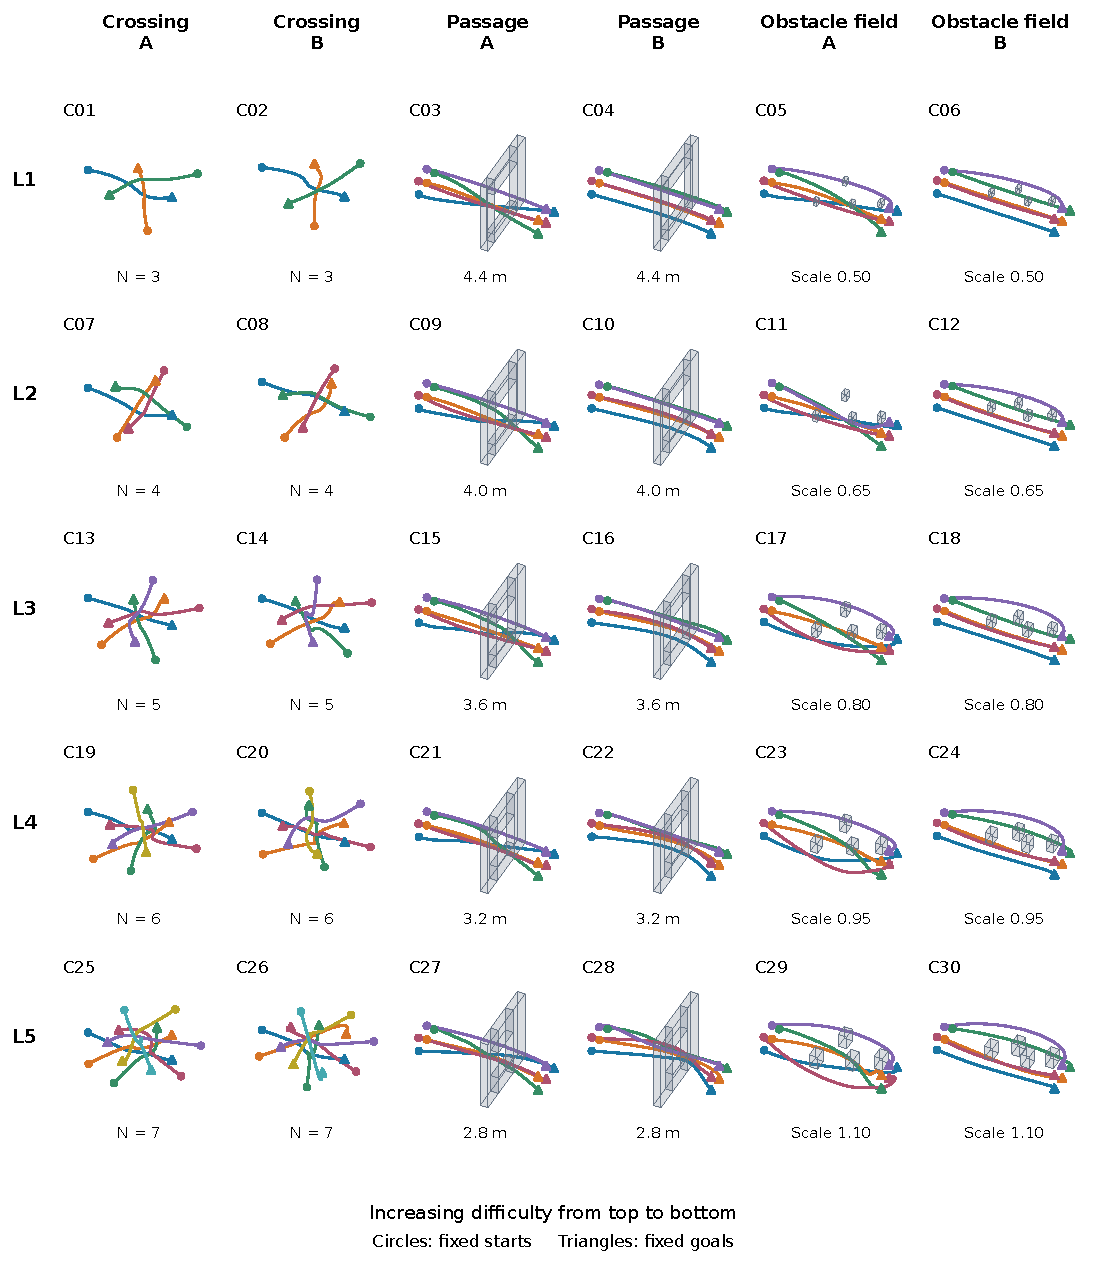
\includegraphics[width=\fulllength,height=20.6cm,keepaspectratio]{figures_rest/all_cases.pdf}
\caption{All 30 rest-to-rest cooperative motions. Rows indicate increasing difficulty; paired columns show the two realizations of each scene family. Small-panel axis ticks are omitted; metric enlarged views appear in Figure~\ref{fig:scenes}.\label{fig:allcases}}
\end{adjustwidth}
\end{figure}
\begin{figure}[p]
\begin{adjustwidth}{-\extralength}{0cm}
\centering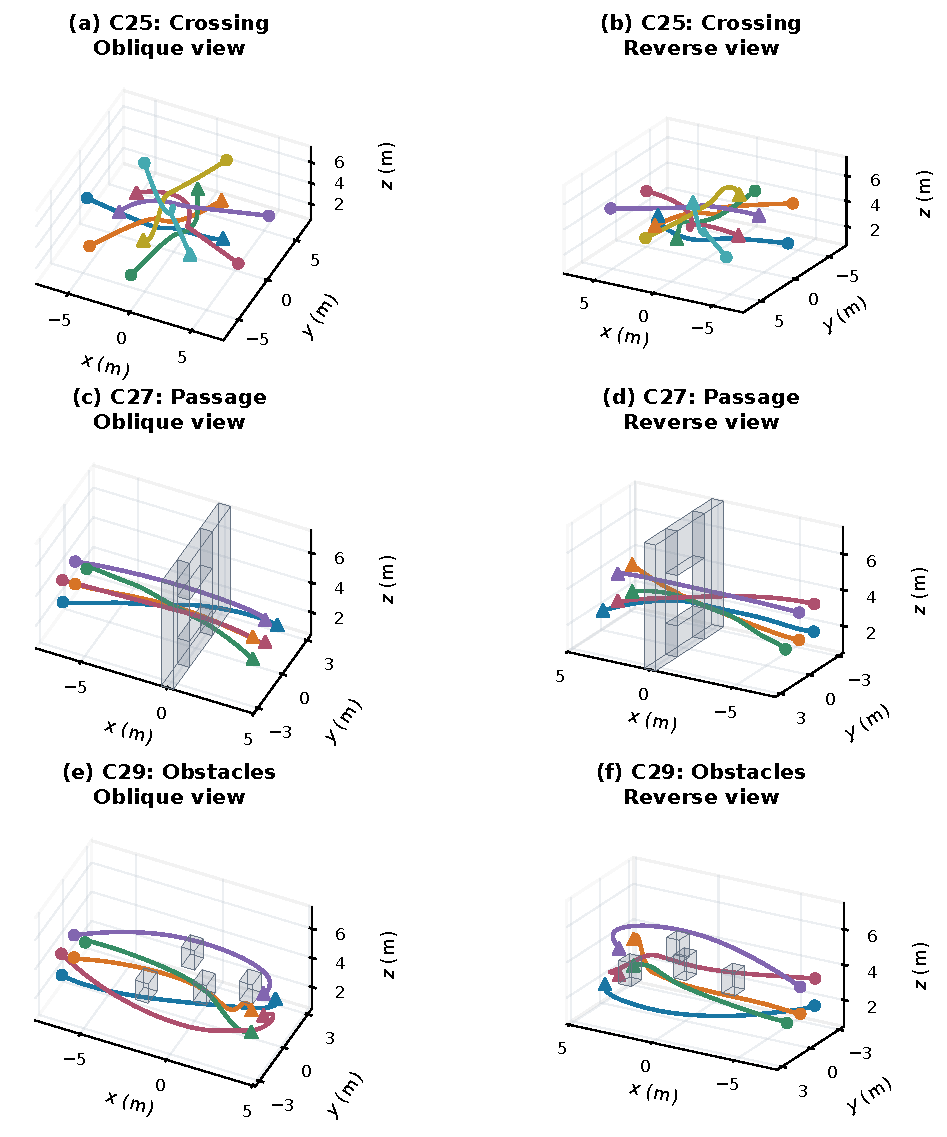
\includegraphics[width=\fulllength,height=20cm,keepaspectratio]{figures_rest/scene_families.pdf}
\caption{Three level-5 examples, each shown from an oblique and reverse view: C25, seven-UAV crossing; C27, five-UAV passage through a 2.8 m opening; and C29, the enlarged obstacle field. Obstacle surfaces are clipped to the displayed window; full geometry is used for planning and checking.\label{fig:scenes}}
\end{adjustwidth}
\end{figure}

C27 illustrates how the spatial reference and final motion differ while maintaining the same task boundaries. Figure~\ref{fig:passage} shows the reference and returned trajectories from an identical camera and gives two orthogonal projections. A projected overlap does not imply a simultaneous three-dimensional collision. Figure~\ref{fig:controls} shows the corresponding continuous velocities and piecewise-constant acceleration controls for all five UAVs.
\begin{figure}[!htb]
\begin{adjustwidth}{-\extralength}{0cm}
\centering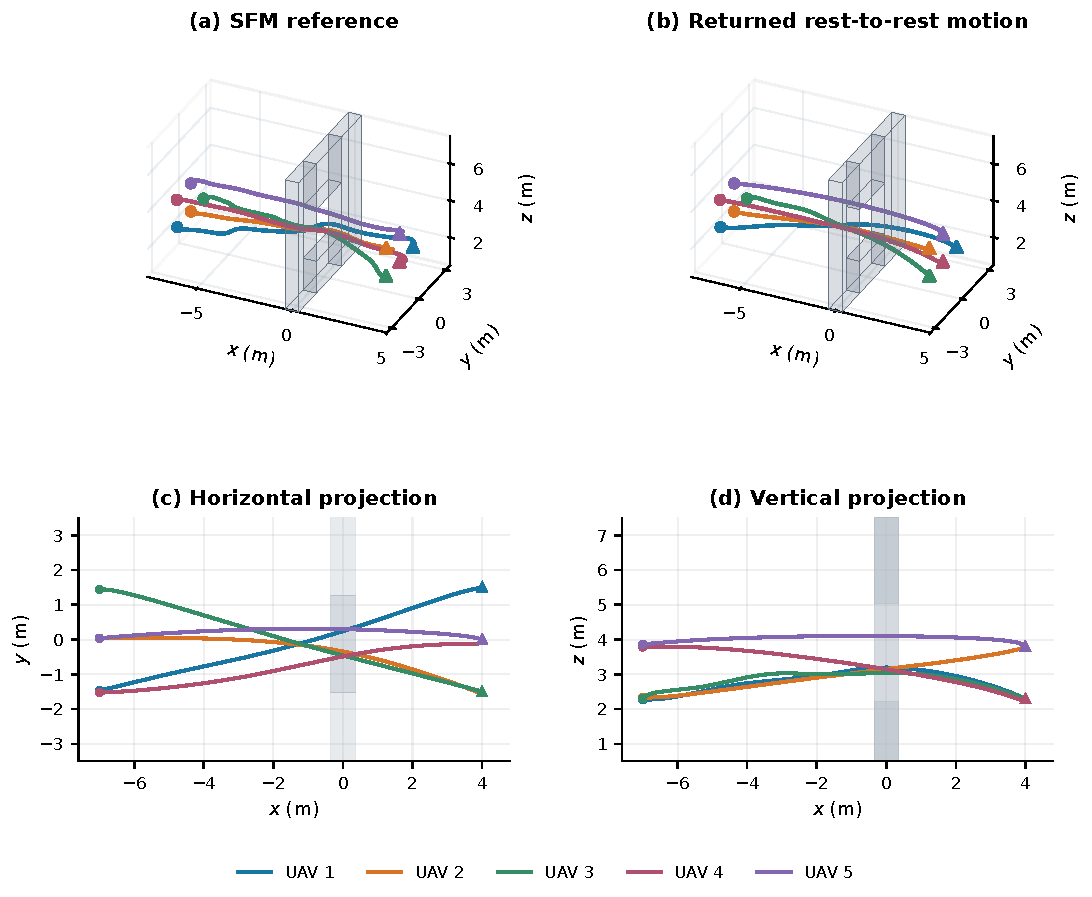
\includegraphics[width=\fulllength]{figures_rest/passage_motion.pdf}
\caption{C27 reference and returned motion, followed by horizontal and vertical projections. Both reference and output have a 12 s horizon and fixed start--goal assignments. Gray planar regions are obstacle projections.\label{fig:passage}}
\end{adjustwidth}
\end{figure}
\begin{figure}[htbp]
\begin{adjustwidth}{-\extralength}{0cm}
\centering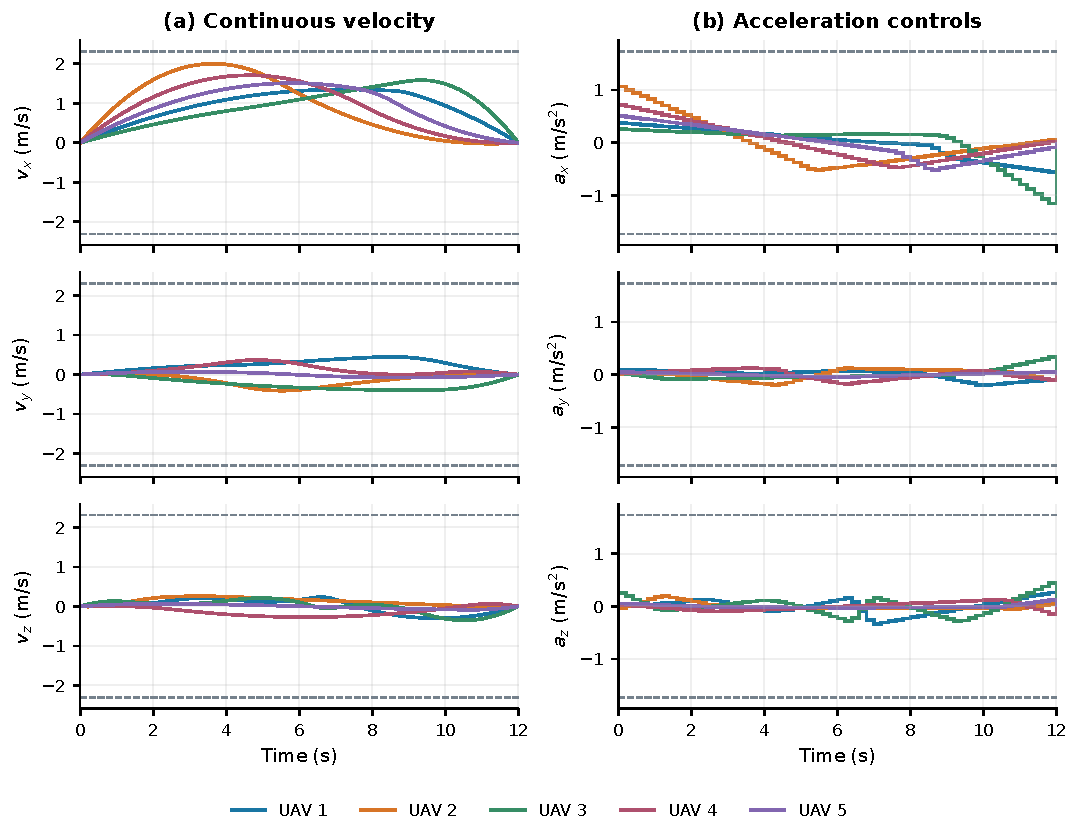
\includegraphics[width=\fulllength]{figures_rest/passage_controls.pdf}
\caption{C27 states and controls. Every velocity curve is continuous and begins and ends at zero. Acceleration is constant on each interval. Dashed lines mark the conservative Cartesian bounds.\label{fig:controls}}
\end{adjustwidth}
\end{figure}

\begin{samepage}
The timing comparison in Figure~\ref{fig:profiles} uses the same admissible scalar rule for SFM and straight geometry. Profile amplitudes depend on their joint path lengths. The common horizon and endpoint-speed conditions provide a consistent timing basis for comparing the two geometric initializations.
\par\end{samepage}
\begin{figure}[htbp]
\begin{adjustwidth}{-\extralength}{0cm}
\centering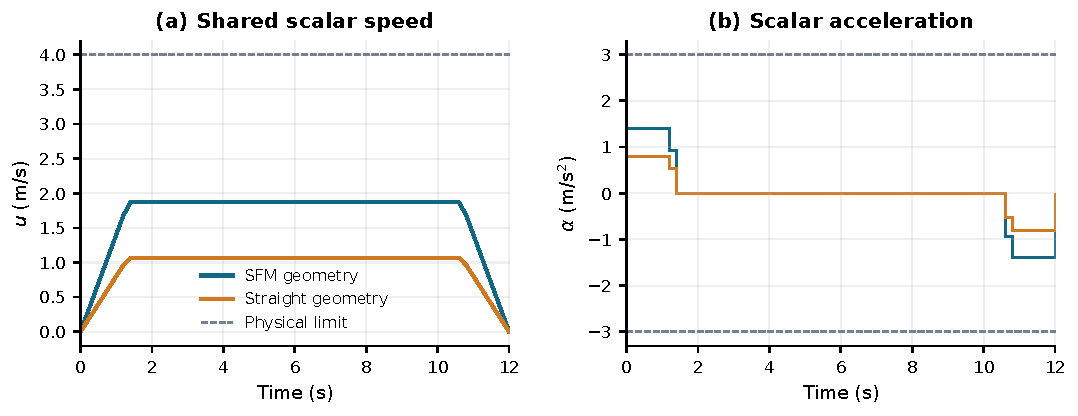
\includegraphics[width=\fulllength]{figures_rest/reference_profiles.pdf}
\caption{C27 scalar reference timing for the two geometric initializations. Both use the same scaled trapezoidal law, prescribed horizon, and zero boundary speeds; dashed lines show the common physical limits.\label{fig:profiles}}
\end{adjustwidth}
\end{figure}

\subsection{Initialization and Recovery Ablations}
Proposed LIOM accepts 30/30 scenes, Straight + LIOM accepts 7/30, and Hard-once accepts 29/30. Figure~\ref{fig:performance} relates these outcomes to per-case CPU time and wall-clock deadlines. Guided reference construction and subsequent guide availability supply useful static detours and passing patterns, increasing success and reducing computation relative to the straight-reference variant. The one-shot formulation is efficient on compatible initial corridors; Proposed LIOM additionally accepts C26 after a second solve.
\begin{figure}[htbp]
\begin{adjustwidth}{-\extralength}{0cm}
\centering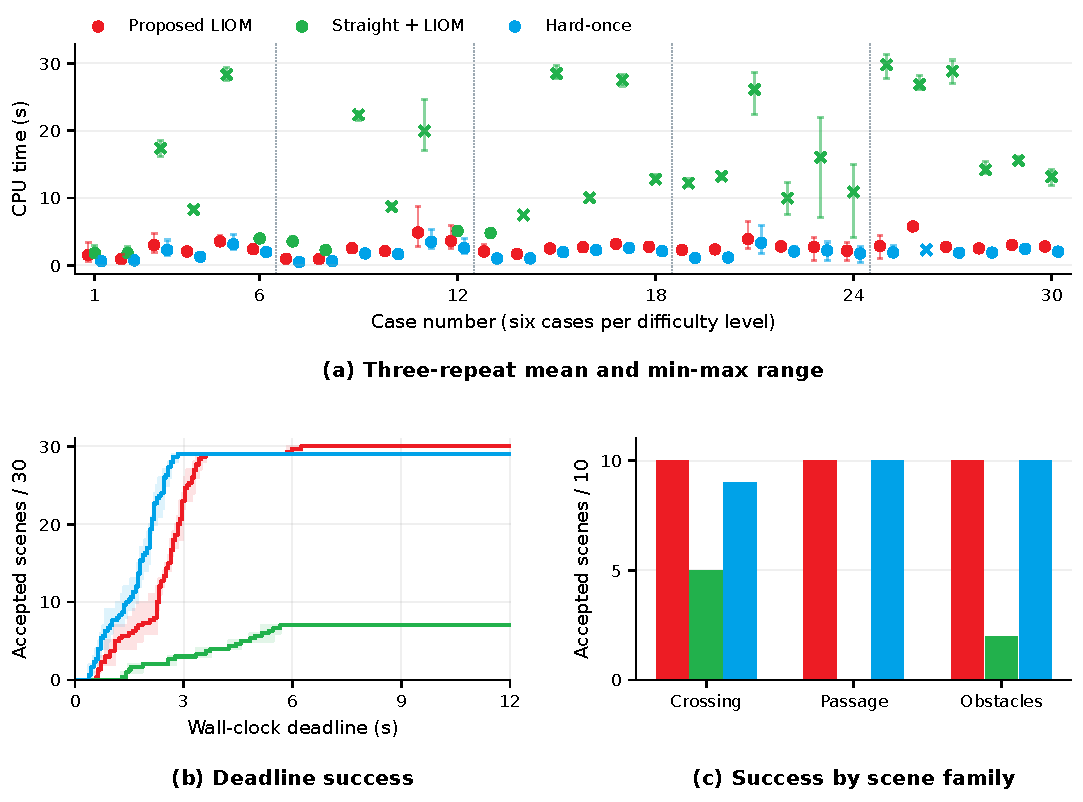
\includegraphics[width=\fulllength]{figures_rest/performance.pdf}
\caption{Initialization and recovery ablation batch. (a) Per-case CPU means and min--max ranges over three repetitions; circles mark acceptance and crosses failure. (b) Accepted scenes by wall-clock deadline, with repetition ranges shaded. (c) Scene-family acceptance. Failed attempts remain in timing statistics.\label{fig:performance}}
\end{adjustwidth}
\end{figure}

The flight duration is fixed at 12 s for every variant. The computation shown in Figure~\ref{fig:performance} precedes execution of that motion.

\subsection{Recovery from Incompatible Initial Corridors}
Proposed LIOM accepts 29 main-benchmark cases after one solve and C26 after two. In C26, the first solve gives $D=1.36\times10^{-2}$ m$^2$ and $S=2.85\times10^{-2}$ m. Both exceed their recovery thresholds. After the weights increase to 2,000 and the corridors are rebuilt, the second candidate reaches $D=4.85\times10^{-9}$ m$^2$ and $S=7.91\times10^{-11}$ m; its reconstructed motion passes the complete-interval checks.

\begin{samepage}
C26's initial hard-box infeasibility was independently confirmed with HiGHS~\cite{huangfu2018}. For the row-scaled linear system $Ax\leq b$, a Phase-I program gives a minimum common relaxation of $1.5175\times10^{-2}$. Nonnegative dual multipliers satisfy $\|A^\top y\|_\infty=2.08\times10^{-17}$ and $b^\top y=-1.5175\times10^{-2}$, with a positive contradiction margin after accounting for finite state bounds. This numerical certificate concerns the selected initial boxes. The accepted second-round trajectory demonstrates recovery of the unchanged physical task through revised local geometry.
\par\end{samepage}

Together, the ablations show the roles of a coordinated reference and the complete recovery procedure. The pressure tests below examine the latter across multiple layouts and degrees of local restriction.

\subsection{Task-Matched Computational Comparison}
\label{sec:external}
Four computational baselines use the common guided reference, hard integration equations, and the same physical task and acceptance tests:
\begin{samepage}
\begin{itemize}
\item \textbf{ASCO-3D}: adaptive risk-range selection of nonlinear collision constraints~\cite{li2021asco}, with range contraction after failed reduced solves and expansion after full-check violations.
\item \textbf{Hard RSC-QP}: spatial boxes and hard relative separating half-spaces based on the relative safe flight corridor principle~\cite{park2021}. This fixed-horizon, centralized variant isolates the hard-corridor component; the cited online planner additionally uses slack and reciprocal avoidance.
\item \textbf{SCP-3D}: successive affine lower bounds on squared separation distances~\cite{augugliaro2012}.
\item \textbf{Direct NLP}: simultaneous enforcement of all nonlinear distance constraints in one solve.
\end{itemize}
\par\end{samepage}
For a reference relative position $\mathbf r^0$ and padded separation $R$, the two affine representations are
\begin{equation}
 \underbrace{\frac{(\mathbf r^0)^\top\mathbf r}{\norm{\mathbf r^0}_2}\geq R}_{\text{Hard RSC-QP}},\qquad
 \underbrace{2(\mathbf r^0)^\top\mathbf r\geq R^2+\norm{\mathbf r^0}_2^2}_{\text{SCP-3D}}.
 \label{eq:baseline-separation}
\end{equation}
Hard RSC-QP uses padded nodes and the common spatial boxes. The other baselines use quarter-interval samples, reachable-displacement padding over $h/8$, and spherical-UAV/AABB distances or their linearizations. Signed distance preserves a penetration gradient for nonlinear intermediate candidates. Each accepted output undergoes the same complete-interval check. These choices compare local constraint representations under identical endpoints, motion limits, and flight duration.

All baselines use the nominal 30 s budget and up to 6,000 inner iterations per solve. ASCO-3D limits each reduced solve to 5 CPU seconds; the others receive the remaining budget. Iterative strategies allow at most 30 solves. ASCO's risk-range parameters are scaled by the ratio of UAV radius to the original covering-disc radius and remain fixed across scenes. Three paired batches rerun Proposed LIOM and Hard-once alongside the four baselines.

\begin{table}[htbp]
\begin{adjustwidth}{-\extralength}{0cm}
\caption{Paired computational comparison on the 30 main-benchmark scenes. Proposed LIOM is the complete method developed in this paper.\label{tab:externalresults}}
\small\setlength{\tabcolsep}{4pt}
\begin{tabularx}{\fulllength}{Yrrrrr}
\toprule Method & Accepted & Within 30 s & CPU mean (s) & Wall mean (s) & Wall P95 (s) \\
\midrule
\textbf{Proposed LIOM} & 30/30 & 30/30 & $1.44\pm0.43$ & $1.31\pm0.40$ & 3.03 \\
Hard-once & 29/30 & 29/30 & $0.92\pm0.31$ & $0.82\pm0.30$ & 2.45 \\
ASCO-3D & 30/30 & 30/30 & $2.14\pm0.53$ & $2.12\pm0.59$ & 6.74 \\
Hard RSC-QP & 30/30 & 30/30 & $1.01\pm0.26$ & $0.91\pm0.25$ & 2.48 \\
SCP-3D & 30/30 & 30/30 & $2.09\pm0.45$ & $2.02\pm0.48$ & 4.87 \\
Direct NLP & 30/30 & 23--29/30 & $11.38\pm2.34$ & $12.01\pm2.75$ & 31.70 \\
\bottomrule\end{tabularx}
\par\vspace{3pt}\footnotesize Counts refer to 30 distinct scenes. The deadline column gives the range across three repetitions; accepted counts are identical in all repetitions. Timing includes every attempt. $\pm$ denotes the SD of the three batch means; P95 uses all 90 attempts per method.

\end{adjustwidth}
\end{table}

Table~\ref{tab:externalresults} shows that Proposed LIOM accepts all scenes at a mean CPU time of 1.44 s, below ASCO-3D, SCP-3D, and Direct NLP. The accepted outputs also meet the 30 s deadline in every repetition. ASCO's constraint selection reduces the cost of the all-distance nonlinear formulation, while the corridor and affine-separation methods exploit the quadratic structure of fixed-horizon translational planning.

Hard RSC-QP accepts all 30 scenes at a mean wall time of 0.91 s, compared with 1.31 s for Proposed LIOM. It also accepts C26 using its initial half-spaces, illustrating how a different local region can resolve a particular incompatibility before iteration begins. The pressure tests examine the complementary requirement: continuing refinement when the local region conflicts with the fixed-horizon task.

The deadline column separates accepted motion from timely completion. Direct NLP returns accepted outputs for all scenes, with 29, 29, and 23 completed within 30 s across the three repetitions; its wall-time P95 is 31.70 s. The remaining methods' accepted main-benchmark outputs finish within 30 s.

\subsection{Recovery under Time and Corridor Pressure}
\label{sec:stress}
The pressure tests use the five-, six-, and seven-UAV crossing layouts C13/C14, C19/C20, and C25/C26. One sweep varies $T_f$ from 8 to 12 s; the other fixes $T_f=12$ s and varies the spatial-box face-growth cap $\ell_s$ from 0.15 to 1.50 m. Both retain $K=60$ and the common physical limits. Each sweep contains 30 settings across six base layouts, with six shared default settings. The growth cap controls local corridor freedom; physical obstacle geometry is unchanged. Proposed LIOM, Hard-once, and Hard RSC-QP use the same cap in each setting, and all failed attempts remain in the counts.

\begin{table}[htbp]
\begin{adjustwidth}{-\extralength}{0cm}
\caption{Acceptance under time and spatial-corridor pressure. Each sweep contains 30 parameter settings across six base layouts.\label{tab:stresssummary}}
\small\begin{tabularx}{\fulllength}{Yrrr}
\toprule Sweep & \textbf{Proposed LIOM} & Hard-once & Hard RSC-QP \\
\midrule
Flight horizon, 8--12 s & 27/30 & 20/30 & 26/30 \\
Spatial-box growth cap, 0.15--1.50 m & 30/30 & 20/30 & 25/30 \\
\bottomrule\end{tabularx}
\end{adjustwidth}
\end{table}


Table~\ref{tab:stresssummary} summarizes acceptance, and Figure~\ref{fig:pressure} locates the recovered settings. In the time sweep, Proposed LIOM accepts 27/30, Hard-once 20/30, and Hard RSC-QP 26/30. Proposed LIOM recovers seven Hard-once failures across four layouts; independent feasibility checks confirm initial hard-box incompatibility in all seven. Nine accepted settings require multiple solves, with at most five. Compared with Hard RSC-QP, the proposed method additionally accepts the six-UAV B and seven-UAV A layouts at 8 s, while Hard RSC-QP alone accepts seven-UAV B at 10 s.

\begin{figure}[!htb]
\begin{adjustwidth}{-\extralength}{0cm}
\centering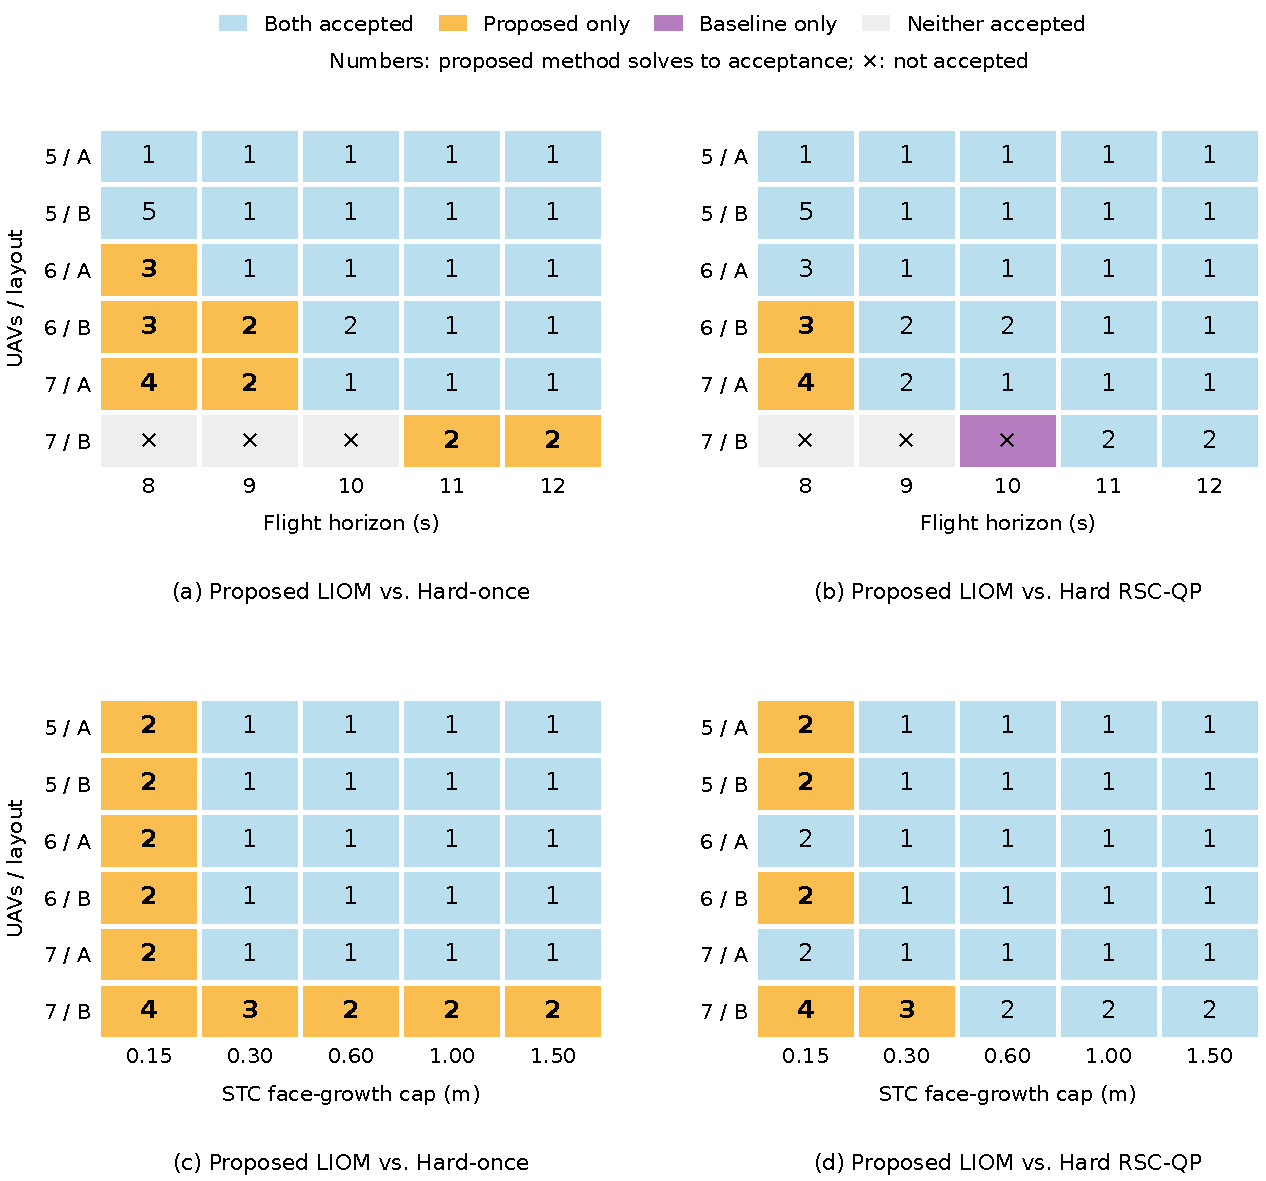
\includegraphics[width=\fulllength]{figures_rest/pressure_sweep.pdf}
\caption{Acceptance across the pressure grids. The upper row varies flight time; the lower row varies spatial-box freedom. A/B denote the two geometric realizations. Colors compare Proposed LIOM with each indicated baseline. Numbers give the proposed method's solves to acceptance; a cross marks its unaccepted attempt.\label{fig:pressure}}
\end{adjustwidth}
\end{figure}

The spatial-box sweep more clearly separates the methods: Proposed LIOM accepts 30/30 settings, Hard-once 20/30, and Hard RSC-QP 25/30. Ten settings have independently confirmed infeasible initial hard-box problems and are recovered in two to four solves. At the smallest cap, every layout requires recovery. All five Hard RSC-QP failures are accepted by the proposed method. Once a hard local region excludes the admissible motion, the low cost of its QP alone offers no route forward. The proposed procedure instead uses intermediate candidates to relocate the corridors while preserving flight time, endpoints, and physical bounds.

The maximum observed wall times among accepted Proposed LIOM runs are 8.51 s in the time sweep and 2.03 s in the box sweep. The seven-UAV B reference exceeds the scalar timing limit at 8 s; at 9 and 10 s, numerical recovery is reached, but the reconstructed outputs do not pass the componentwise motion checks within the stopping budget.

Together, the sweeps demonstrate recovery across multiple layouts and degrees of local restriction. Compatible initial geometry permits a short hard-corridor solve. When that compatibility is lost, the complete recovery procedure provides intermediate candidates for geometry updates and subsequent acceptance at the unchanged flight horizon.


\section{Conclusion}
This paper has developed a lightweight feasibility-recovery framework for fixed-horizon multi-UAV cooperative flight trajectory optimization in high-conflict regions. Spatial and relative corridors provide conservative linear restrictions, while separate kinematic and relative-box penalties preserve a nonempty quadratic subproblem under endpoint-compatible spatial boxes. Intermediate candidates support successive corridor reconstruction and bounded penalty updates within the prescribed flight horizon. Closed-form endpoint control correction and exact integration then produce continuous-velocity, rest-to-rest motion, with complete-interval checks determining final acceptance.

Controlled simulations establish second-scale planning for the tested small teams in known, static environments. The paired comparison demonstrates lower mean computation than the tested nonlinear and sequential distance-linearization baselines, alongside the efficiency of compatible hard separating corridors. Time and corridor-pressure sweeps show the proposed method's ability to recover additional accepted motions across multiple layouts. Independent checks of initial hard-box infeasibility connect these results to the resolution of local geometric conflicts. The framework thereby combines tractable local optimization with a practical route from incompatible initial corridors to accepted cooperative flight at a fixed completion time.

\par
\authorcontributions{Conceptualization, Z.Y., W.T. and Z.W.; software, Y.L. and Z.Y.; investigation, Z.Y. and B.Q.; data curation, B.Q.; writing---original draft preparation, Y.L., B.Q. and Z.W.; supervision, W.T. and Z.W.; funding acquisition, W.T. and Z.W.}
\funding{This research was funded by the Fundamental Research Funds for the Central Universities, grant number 40500-20104-222624.}
\institutionalreview{Not applicable.}
\informedconsent{Not applicable.}
\dataavailability{The data supporting the findings of this study are available from the corresponding author upon reasonable request.}
\conflictsofinterest{The authors declare no conflict of interest.}
\begin{adjustwidth}{-\extralength}{0cm}
\reftitle{References}
% Keep the publisher's note with the bibliography after the reference update.
\AtEndEnvironment{thebibliography}{\enlargethispage{3\baselineskip}}
\bibliography{references}
\PublishersNote{}
\end{adjustwidth}
\end{document}
